\documentclass[xcolor=x11names,compress,mathserif,handout]{beamer}

\newcommand{\hackspace}{\hspace{4.2mm}}
\newcommand{\showstudent}[1]{}
\newcommand\hmmax{0}
\newcommand\bmmax{0}


\usepackage{../includes/MarkMathCmds}





% talk/author information
\newcommand{\authorname}{Mark van der Wilk}
\newcommand{\authoremail}{m.vdwilk@imperial.ac.uk}
\newcommand{\authoraffiliation}{
  Department of Computing\\Imperial
  College London}
\newcommand{\authortwitter}{markvanderwilk}
\newcommand{\slidesettitle}{\imperialBlue{Bayesian Linear Regression}}
\newcommand{\footertitle}{Measuring Generalisation}
\newcommand{\location}{Imperial College London}
\newcommand{\talkDate}{November 16, 2021}



\date{\imperialGray{\talkDate}}

% load defaults
\input{../includes/header.tex}


\input{../includes/titlepage.tex}
\linespread{1.2} 



%%%%%%%%%%%%%%%%%%%%%%%%%%%%%%%%%%%%%%%%%
\begin{frame}{Reference}
  \begin{center}
    \emph{Mathematics for Machine Learning:}\\[3mm]
    \emph{\url{https://mml-book.com}}\\[3mm]
    \cemph{Chapter 9}
  \end{center}
\end{frame}


\begin{frame}{Probabilistic Models}
\emph{Probabilistic model}: Model of the data is a probability distribution. \pause \\
\vspace{-0.4cm}
\begin{align*}
y_n = f(\vx_n; \vtheta) + \epsilon_n &&
\epsilon_n \sim \NormDist{0, \sigma^2}
\end{align*} \pause
We can now also estimate the \emph{unpredictability} of our problem:
  \begin{figure}
    \centering
    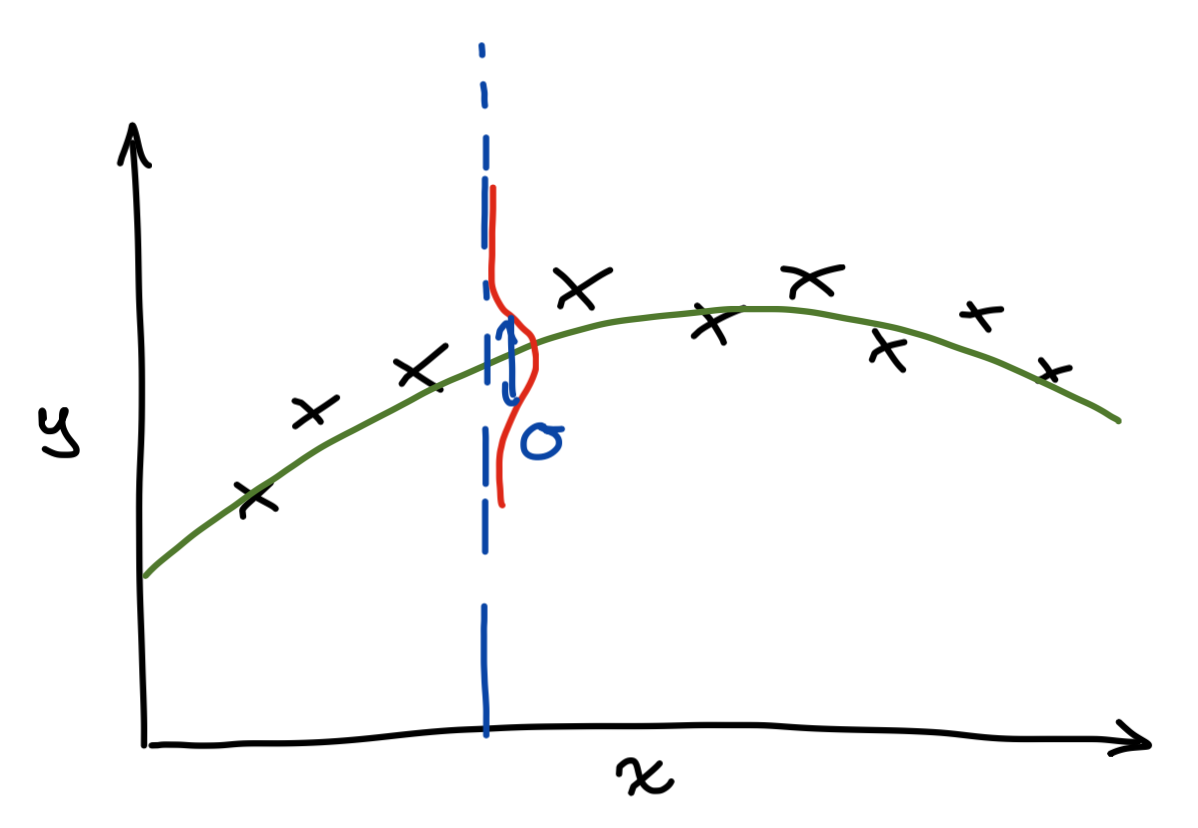
\includegraphics[width = 0.45\hsize]{./figures-l11-blr/regression-noise.png}
  \end{figure}
\vspace{-0.3cm}
\begin{align}
(\vtheta^*, {\sigma^2}^*) = \argmax {}_{\vtheta, \sigma^2} \log p(\vy|\vtheta, \sigma^2, X)
\end{align}

Unpredictability remains even if we \emph{know} underlying function. \\
Goes by many names... e.g.~\emph{aleatoric uncertainty}. \pause
\end{frame}


\begin{frame}{Uncertainty in Parameters/Function}
Aren't we also uncertain when we have a lack of data?
  \begin{figure}
    \centering
    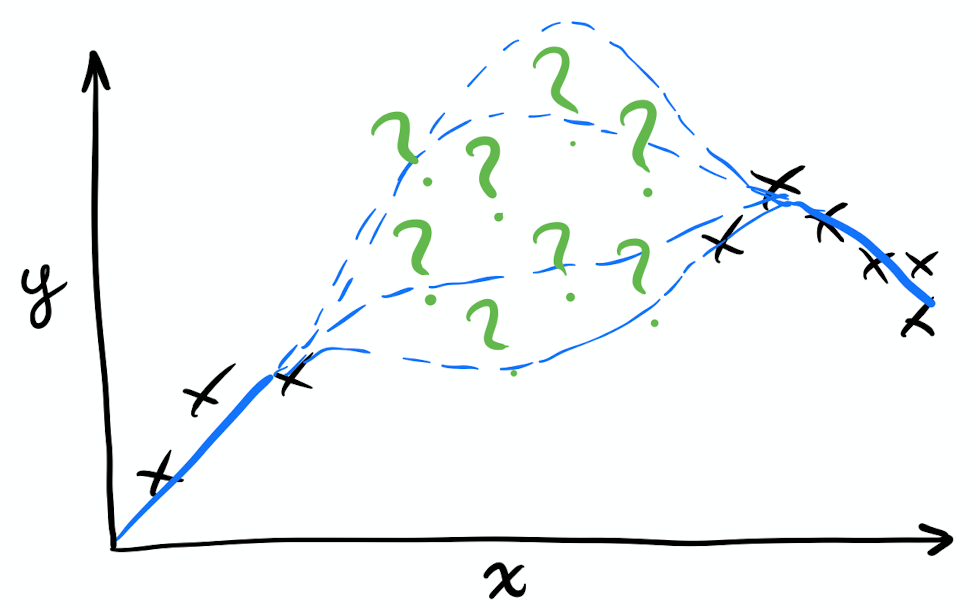
\includegraphics[width = 0.5\hsize]{./figures-l11-blr/regression-uncertainty.png}
  \end{figure}
\vspace{-0.3cm}
This is uncertainty in the parameters that define the function! \\
Also goes by many names... e.g.~\emph{epistemic uncertainty}.
\end{frame}


\begin{frame}{Quantifying Uncertainty with Bayesian Inference}
If we knew that for a series of problems, our parameters $\vtheta$ were sampled from $p(\vtheta)$, then Bayes' rule would give us the probability distribution after observing our data $\vy$:
\begin{align}
\underbrace{p(\vtheta|\vy)}_{\text{posterior}} = \frac{\overbrace{p(\vy|\vtheta)}^{\text{likelihood}}\overbrace{p(\vtheta)}^{\text{prior}}}{\underbrace{p(\vy)}_{\text{evidence}}}
\end{align}

\begin{itemize}
\item Allows us to quantify uncertatinty in parameters $\vtheta$.
\item Bayesian inference makes a leap of faith: Choose a prior and assume this is the correct one.
\item Choosing priors is important $\implies$ Probabilistic Inference (Spring).
\end{itemize}
\end{frame}





\begin{frame}{Example}
  \begin{figure}
    \centering 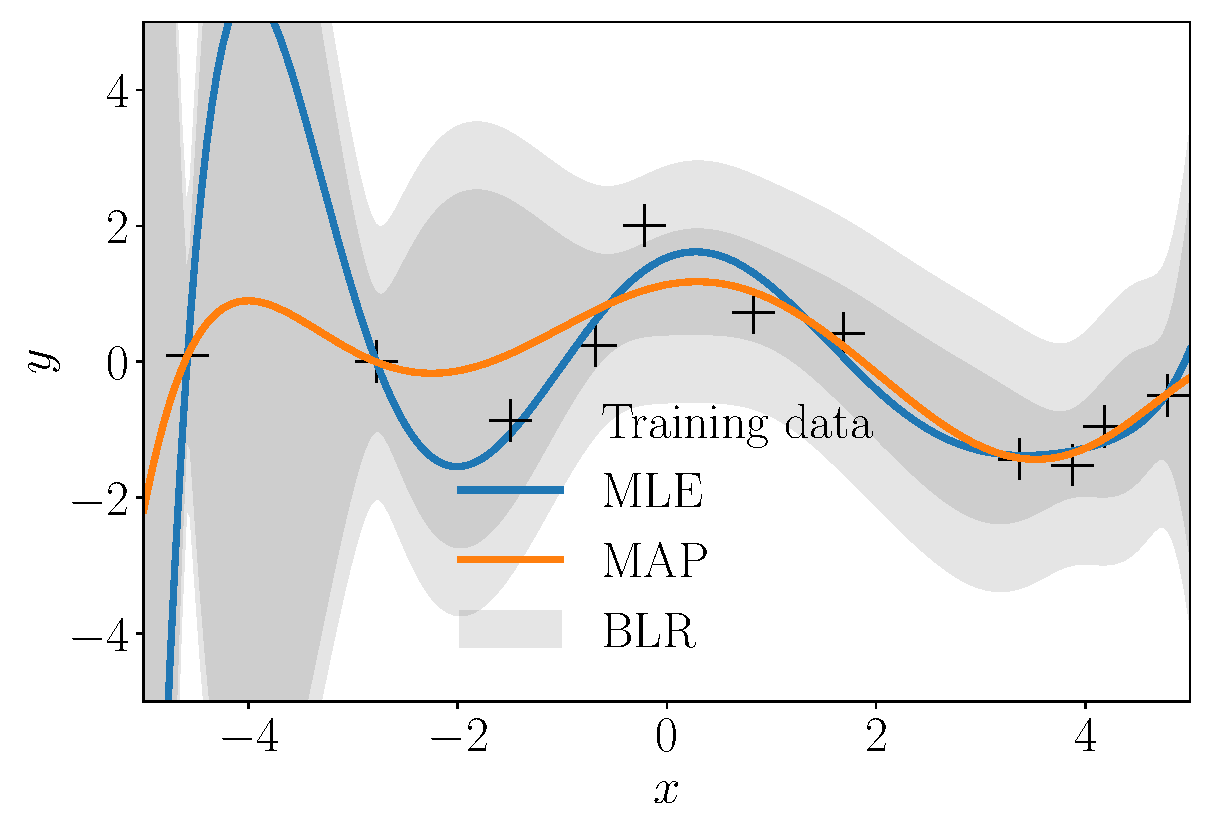
\includegraphics[width =
    0.48\hsize]{./figures-l11-blr/demo_regression_posterior_with_mle_map_7}
    \hfill 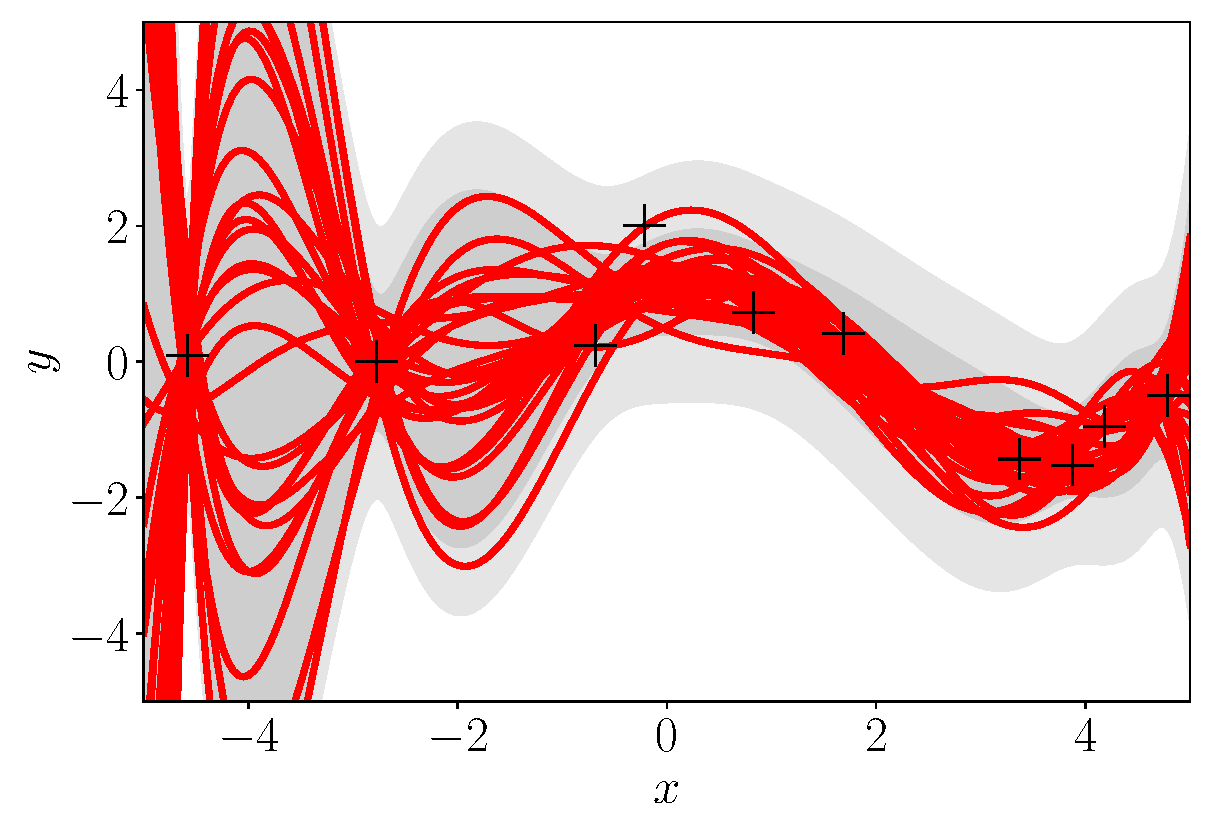
\includegraphics[width =
    0.48\hsize]{./figures-l11-blr/demo_regression_posterior_samples_7}
  \end{figure}

  \begin{itemize}
  \item Light-gray: uncertainty due to noise \\(aleatoric uncertainty / unpredictability)
  \item Dark-gray: uncertainty due to parameter uncertainty \\ (epistemic uncertainty)
    \pause
  \item Right: Plausible functions under the parameter distribution
    (every single parameter setting describes one function)
  \end{itemize}
\end{frame}


\begin{frame}
\frametitle{Distribution over Functions}
% Good thing: Bayesian linear regression induces a probability
% distribution over functions
Consider a linear regression setting 
\begin{align*}
y &= f(x) + \epsilon = a + bx + \epsilon\,,\quad
  \epsilon\sim\gauss{0}{\sigma_n^2}\\
  p(a,b) &= \gauss{\vec 0}{\mat I}
          \\
 \phantom{ [a_i, b_i] \sim p(a,b) }
\end{align*}
\begin{figure}
  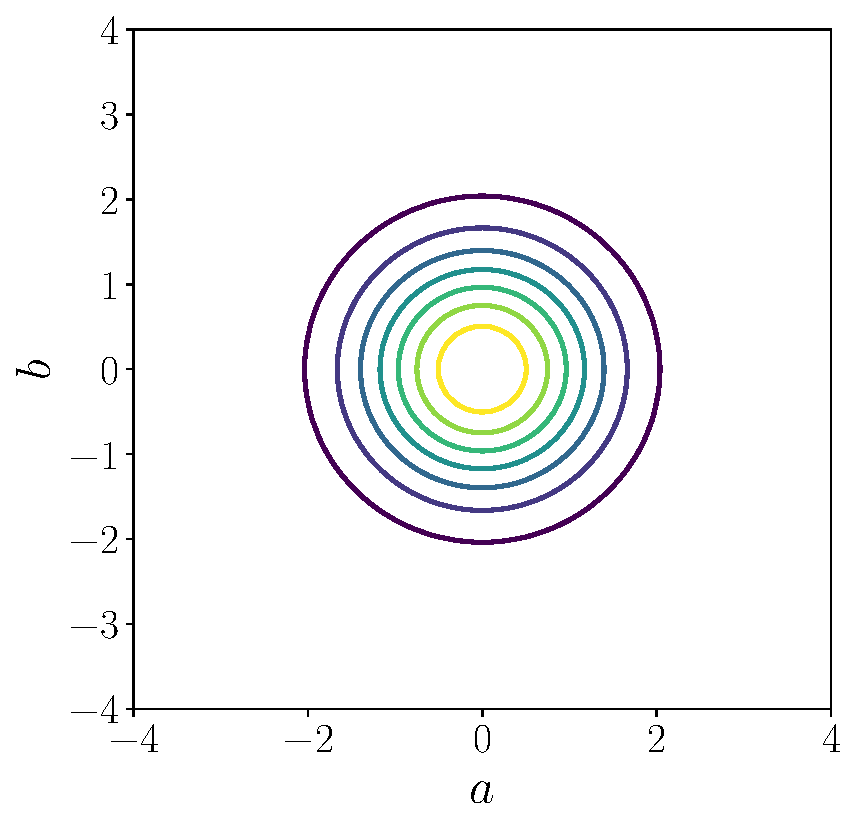
\includegraphics[height = 5cm]{./figures-l11-blr/parameter_prior}
\end{figure}
\end{frame}



\begin{frame}
\frametitle{Sampling from the Prior over Functions}
% Good thing: Bayesian linear regression induces a probability
% distribution over functions
Consider a linear regression setting 
\begin{align*}
y &=f(x) + \epsilon = a + bx + \epsilon\,,\quad
  \epsilon\sim\gauss{0}{\sigma_n^2}\\
p(a,b)& = \gauss{\vec 0}{\mat I}\\
  f_i(x) &= a_i + b_ix, \quad [a_i,b_i]\sim p(a,b)
\end{align*}


\onslide*<1>{\begin{figure}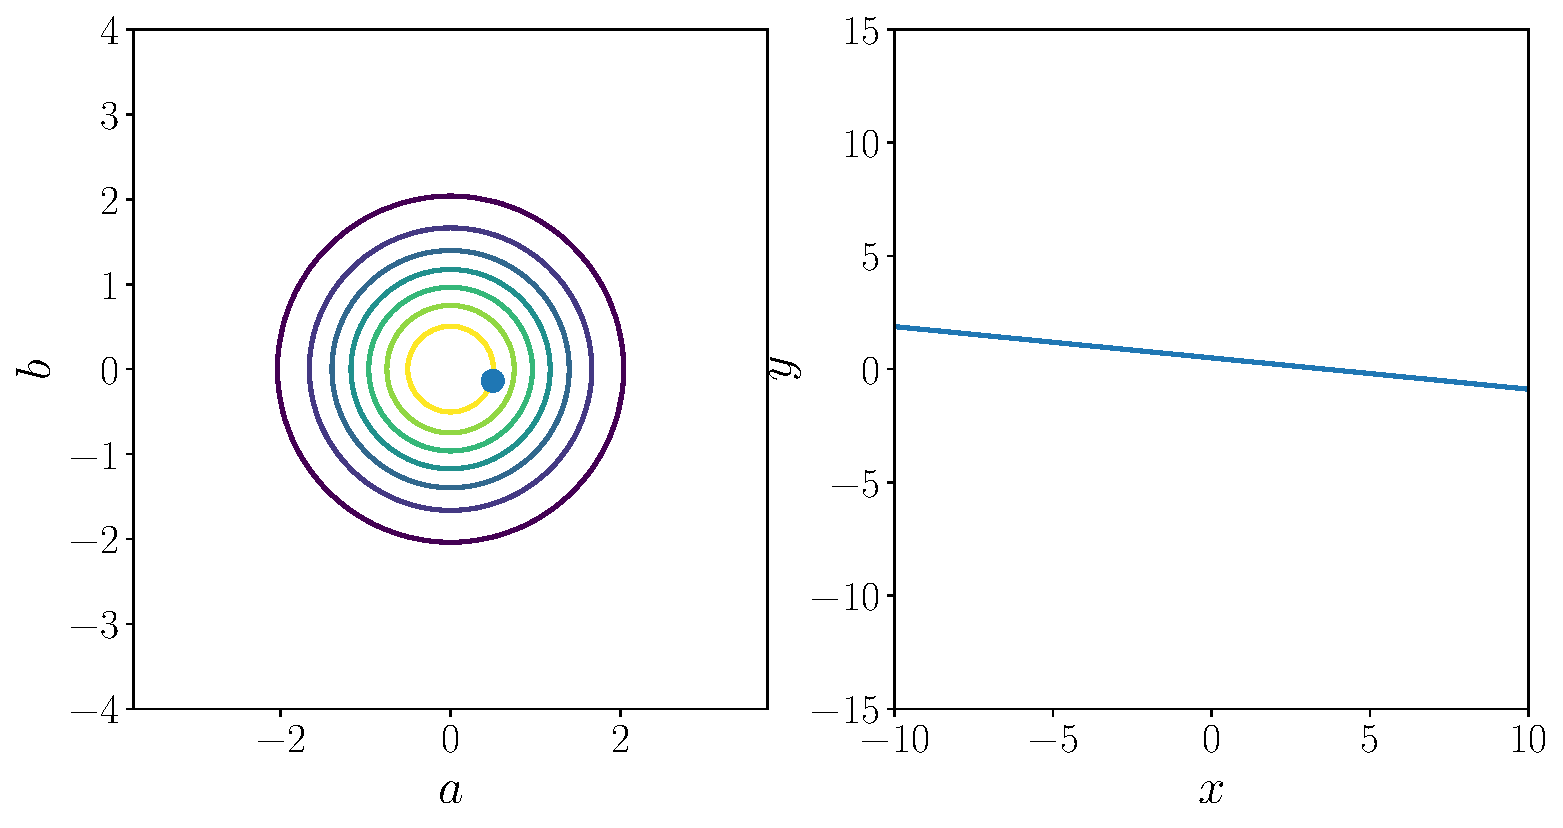
\includegraphics[height = 5cm]{./figures-l11-blr/animation-param-func-dual/prior_samples_fct_distr_0}\end{figure}}
\onslide*<2>{\begin{figure}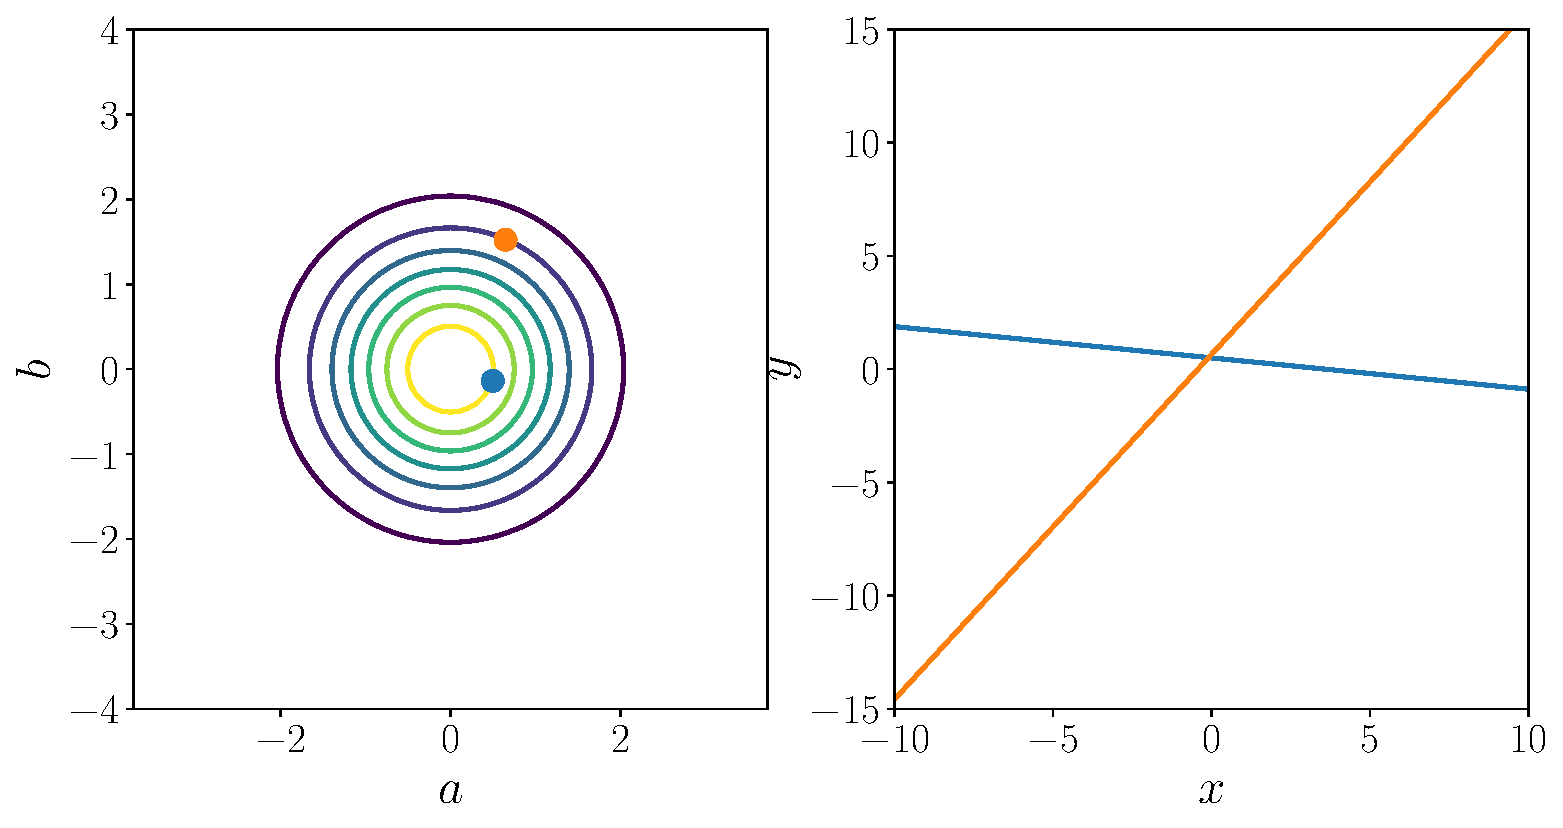
\includegraphics[height = 5cm]{./figures-l11-blr/animation-param-func-dual/prior_samples_fct_distr_1}\end{figure}}
\onslide*<3>{\begin{figure}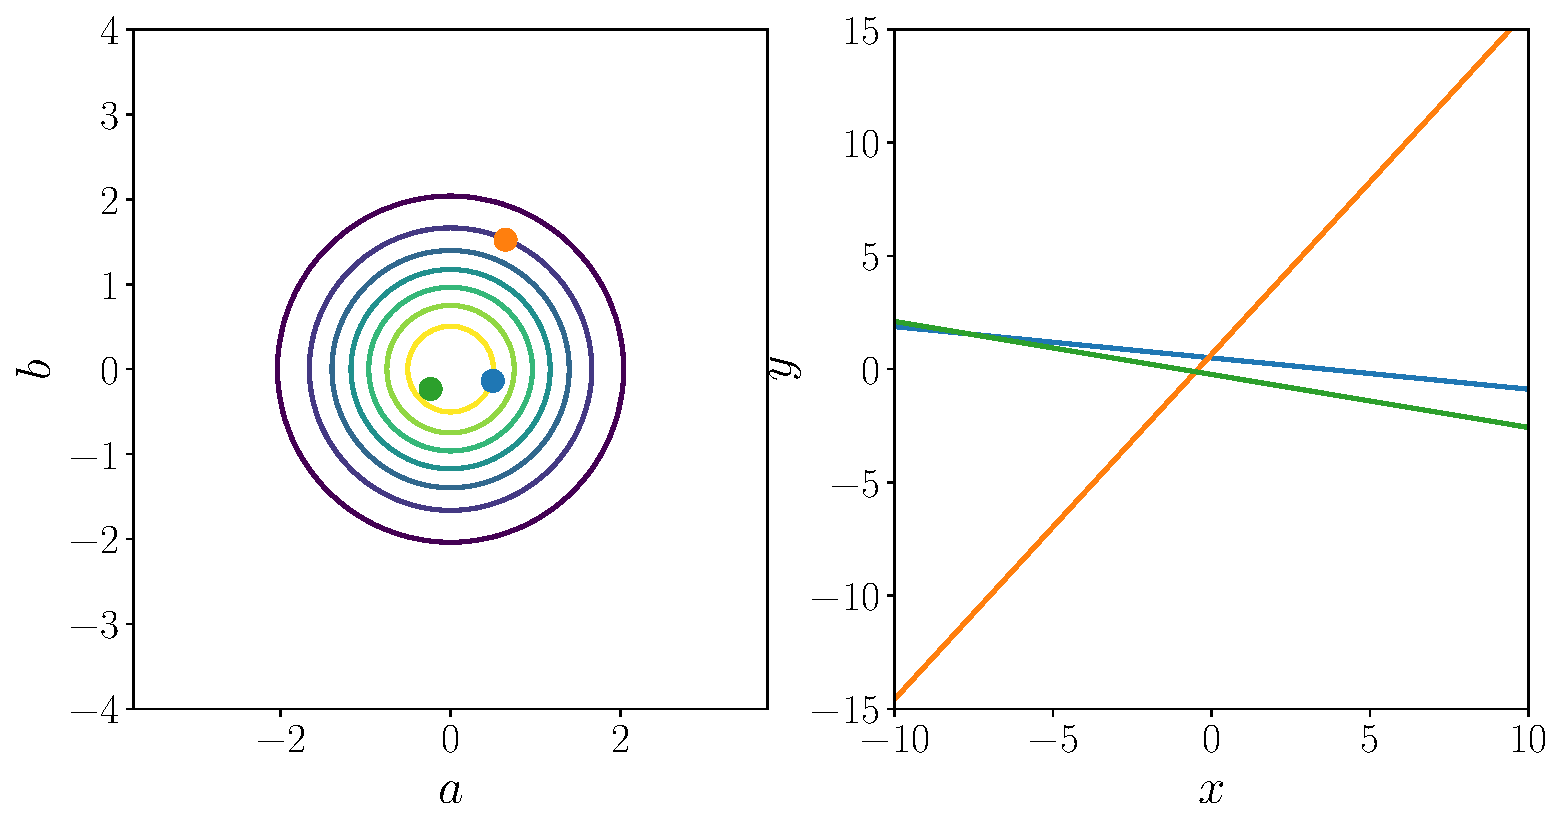
\includegraphics[height = 5cm]{./figures-l11-blr/animation-param-func-dual/prior_samples_fct_distr_2}\end{figure}}
\onslide*<4>{\begin{figure}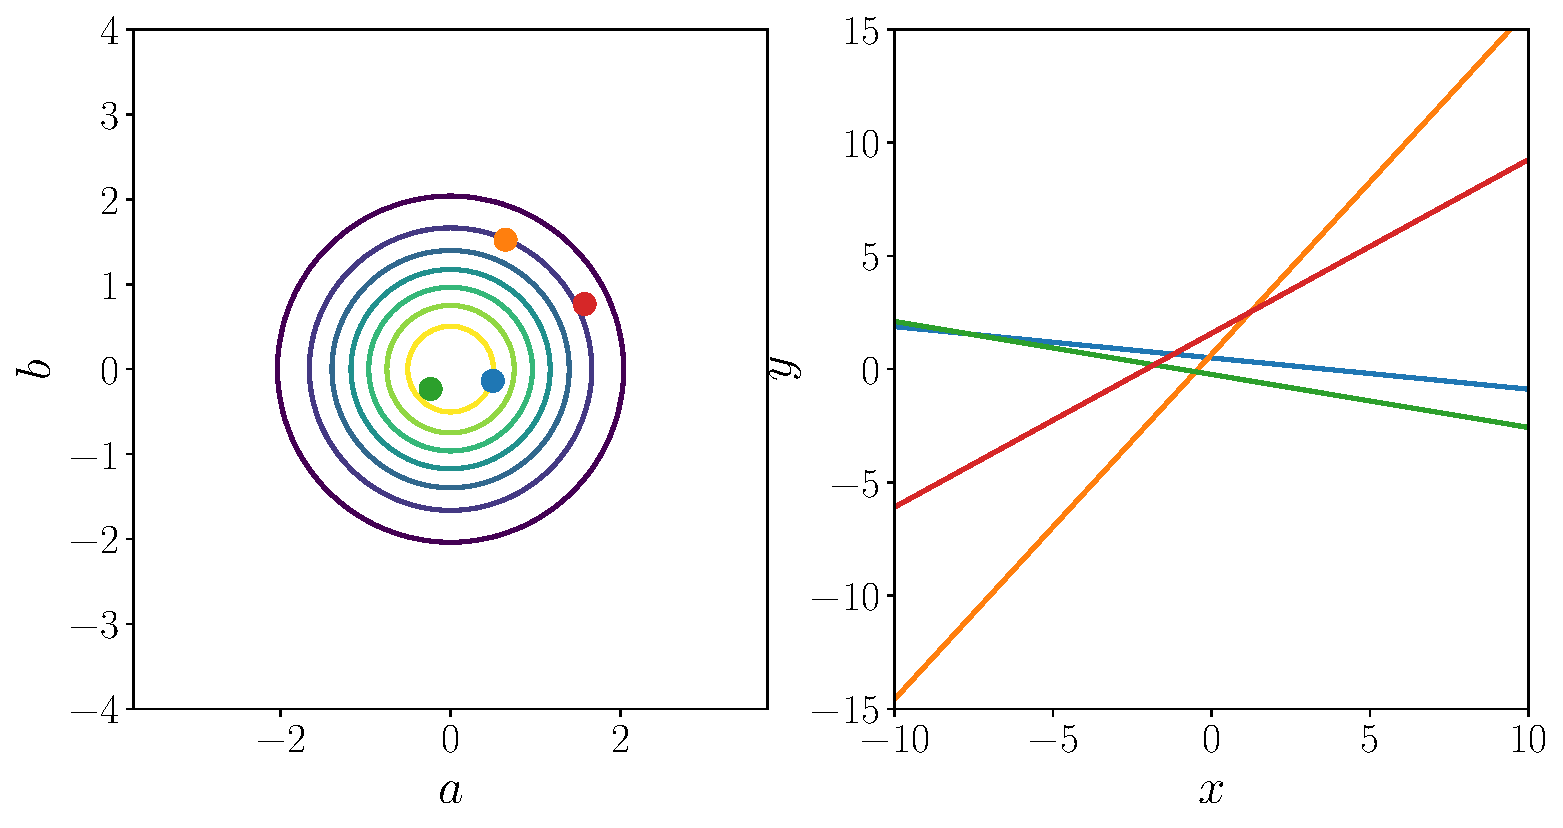
\includegraphics[height = 5cm]{./figures-l11-blr/animation-param-func-dual/prior_samples_fct_distr_3}\end{figure}}
\onslide*<5>{\begin{figure}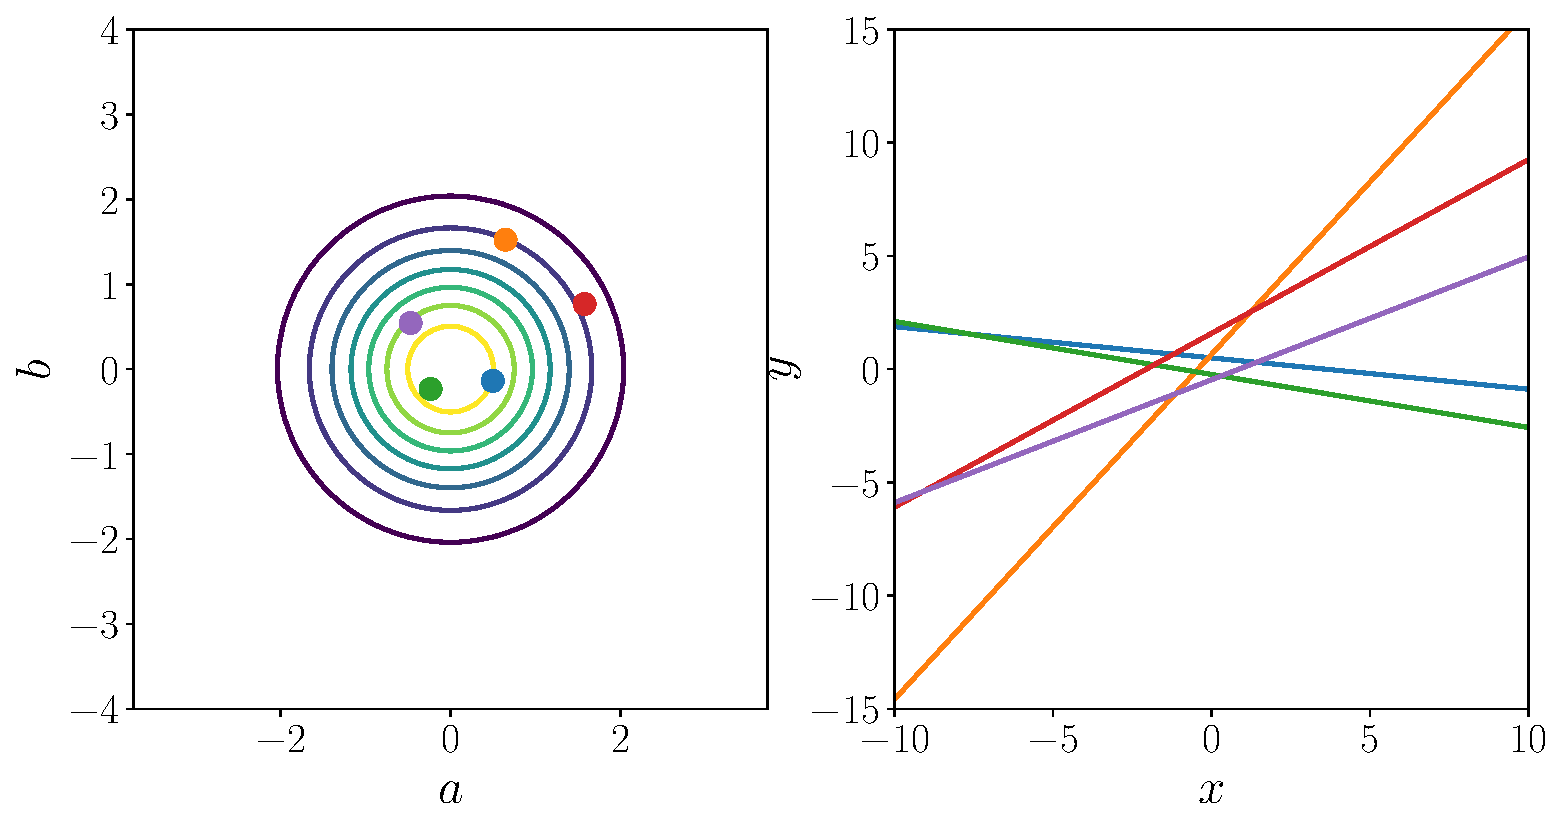
\includegraphics[height = 5cm]{./figures-l11-blr/animation-param-func-dual/prior_samples_fct_distr_4}\end{figure}}
\onslide*<6>{\begin{figure}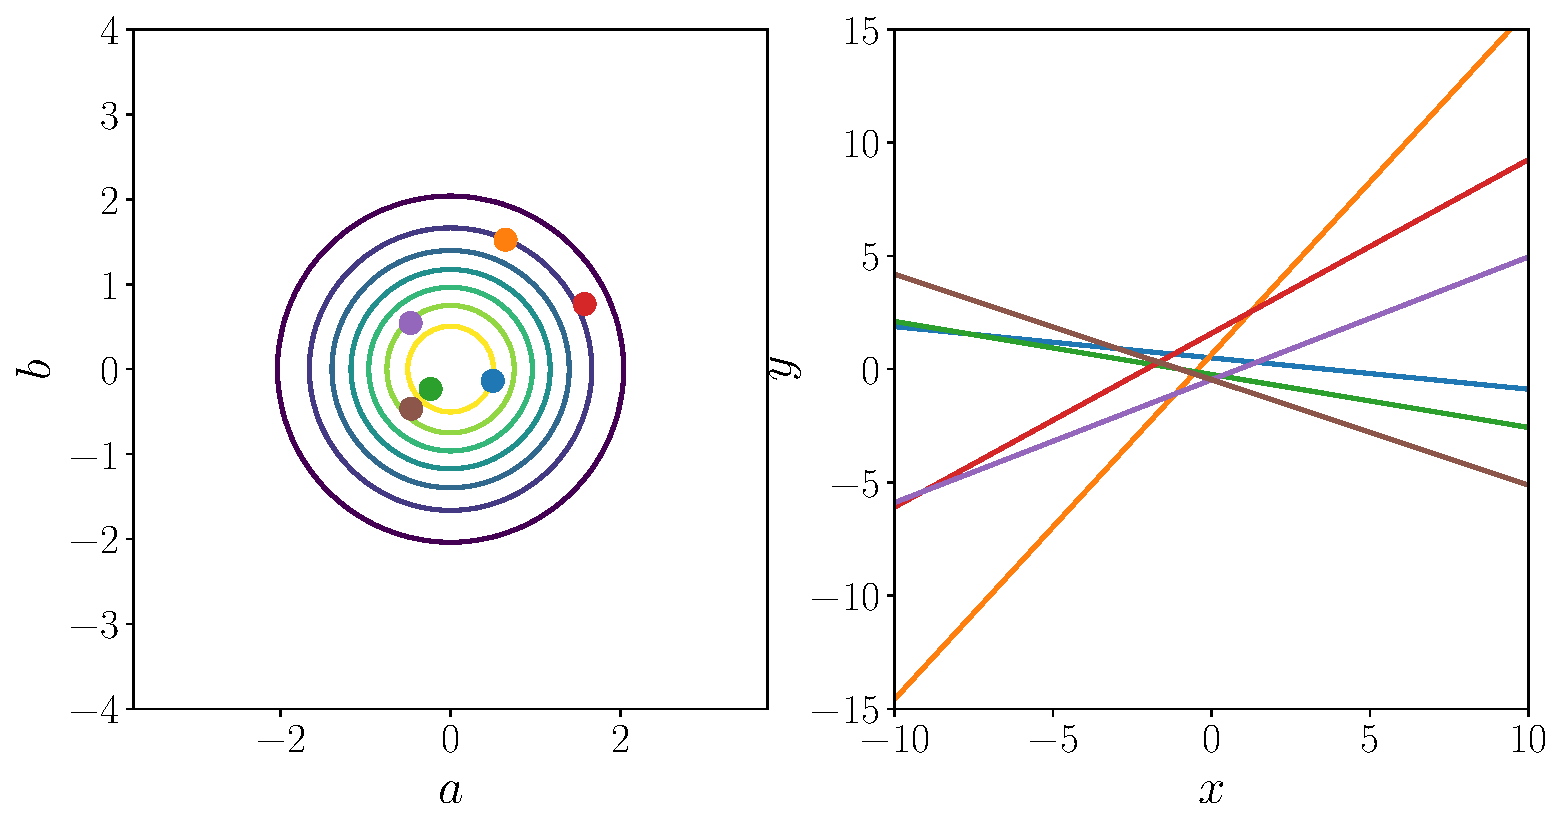
\includegraphics[height = 5cm]{./figures-l11-blr/animation-param-func-dual/prior_samples_fct_distr_5}\end{figure}}
\onslide*<7>{\begin{figure}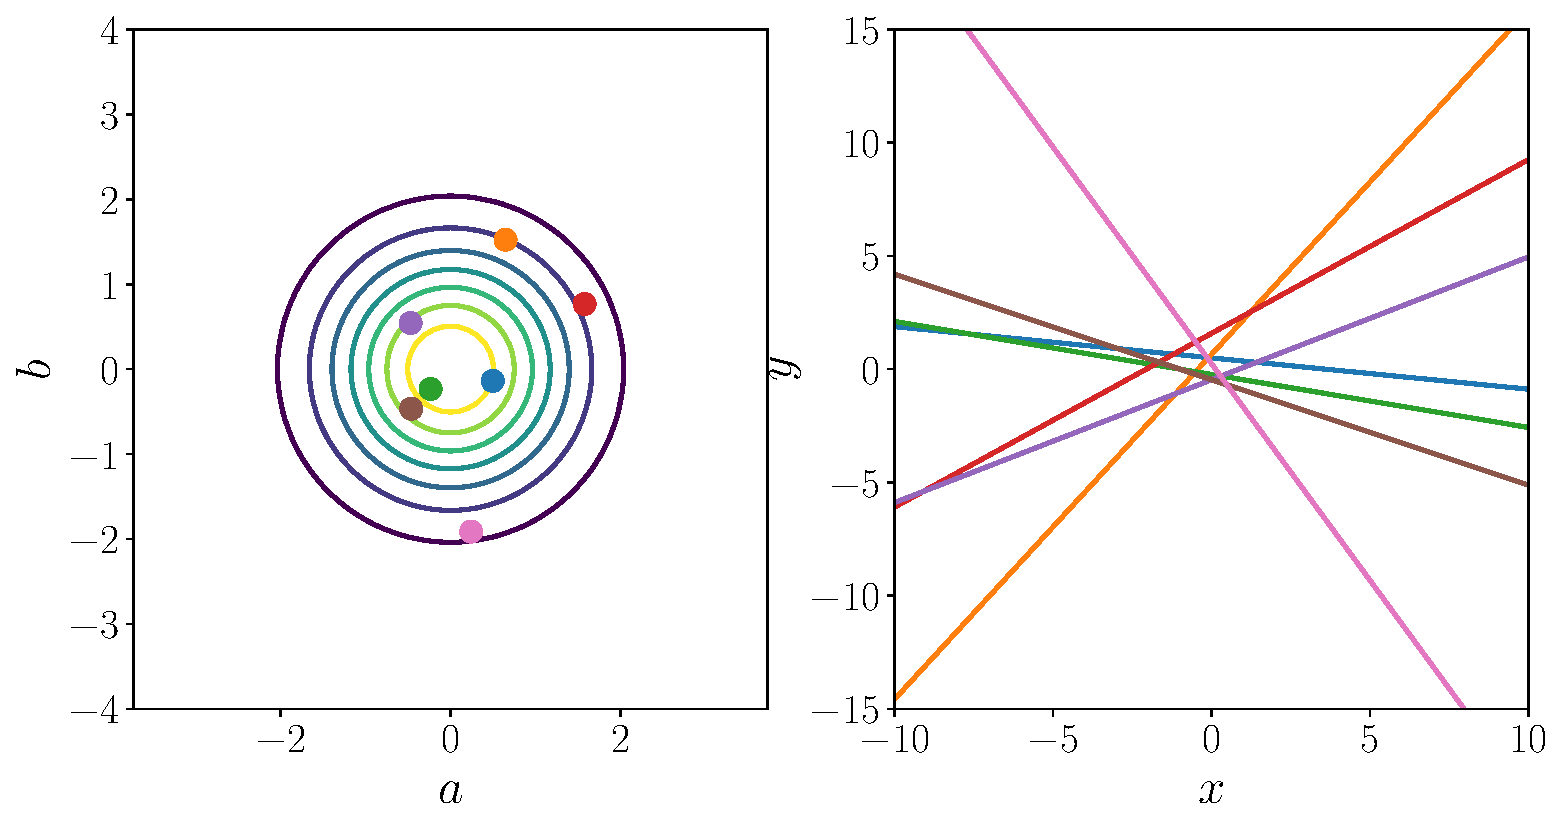
\includegraphics[height = 5cm]{./figures-l11-blr/animation-param-func-dual/prior_samples_fct_distr_6}\end{figure}}
\onslide*<8>{\begin{figure}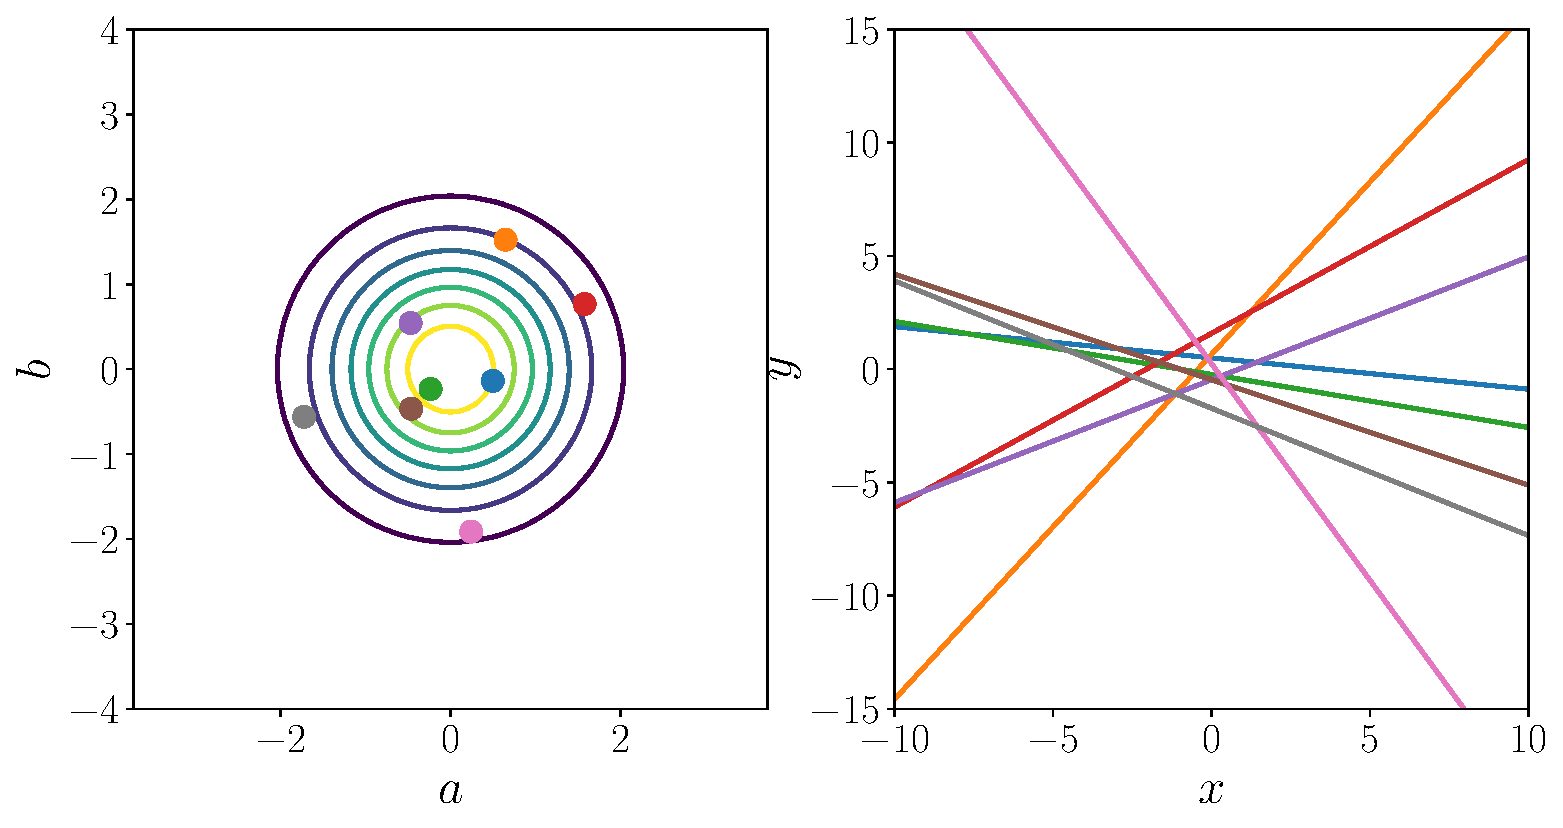
\includegraphics[height = 5cm]{./figures-l11-blr/animation-param-func-dual/prior_samples_fct_distr_7}\end{figure}}
\onslide*<9>{\begin{figure}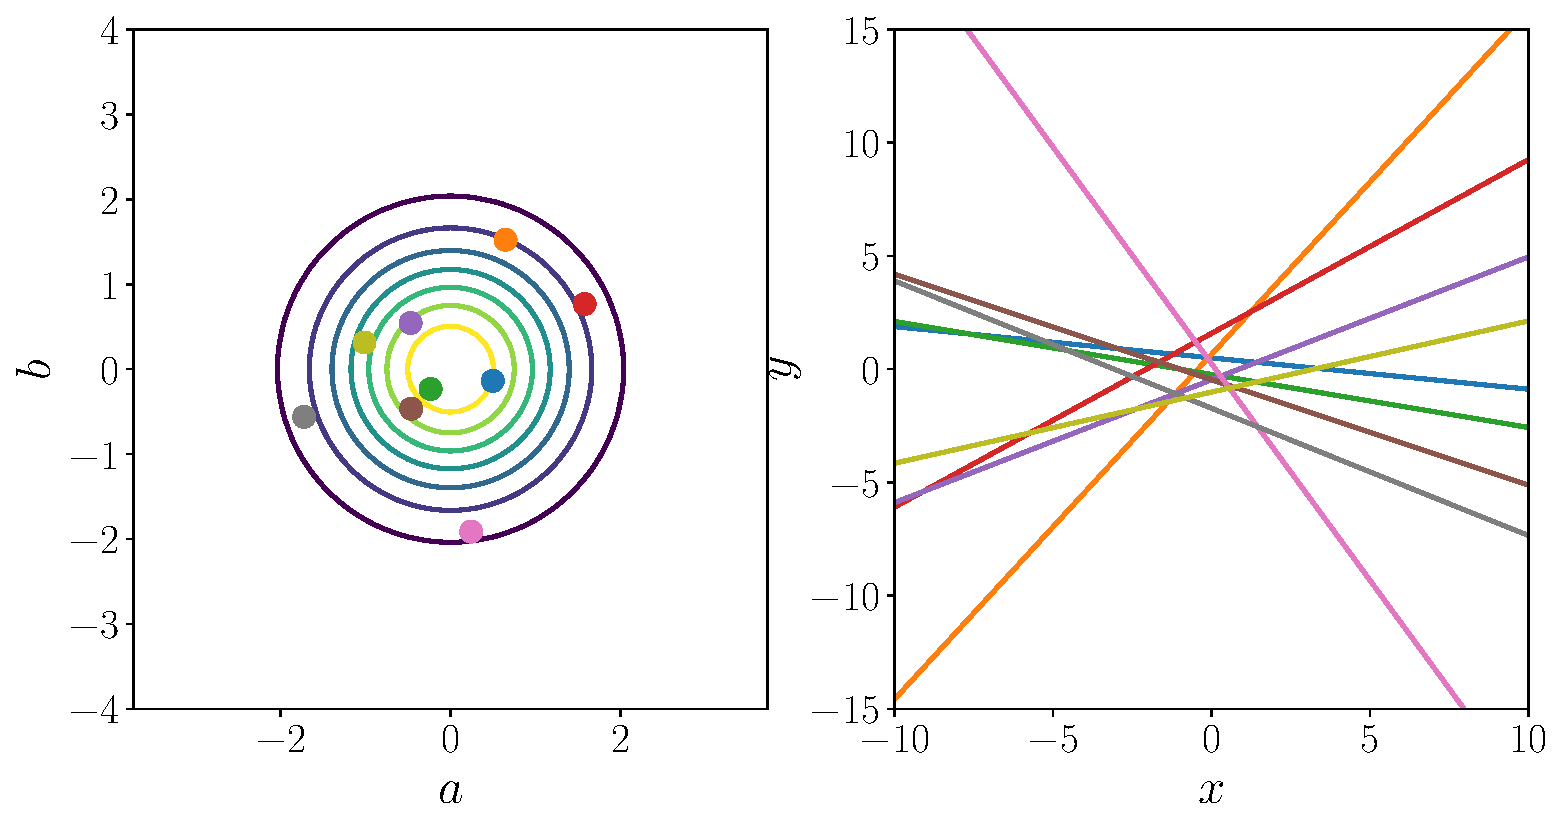
\includegraphics[height = 5cm]{./figures-l11-blr/animation-param-func-dual/prior_samples_fct_distr_8}\end{figure}}
\onslide*<10>{\begin{figure}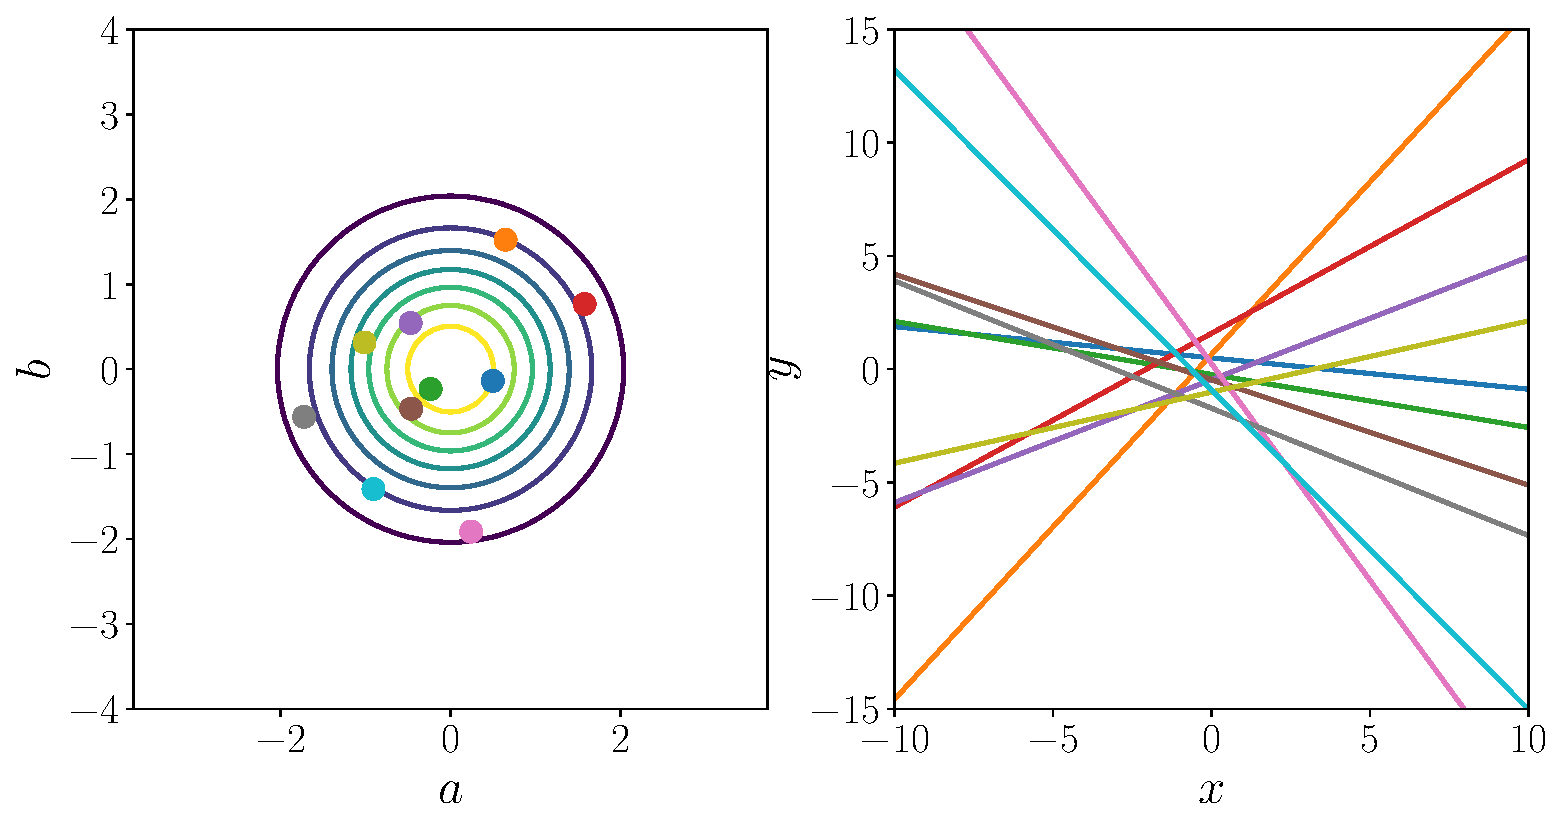
\includegraphics[height = 5cm]{./figures-l11-blr/animation-param-func-dual/prior_samples_fct_distr_9}\end{figure}}
\end{frame}

% %%%%%%%%%%%%%%%%%%%%%%%%%%%%%%%%%%%%%%
\begin{frame}
\frametitle{Sampling from the Posterior  over Functions}
% Good thing: Bayesian linear regression induces a probability
% distribution over functions
Consider a linear regression setting 
\begin{align*}
y &= f(x) + \epsilon =a + bx + \epsilon\,,\quad
  \epsilon\sim\gauss{0}{\sigma_n^2}\\
  p(a,b)& = \gauss{\vec 0}{\mat I}\\
  \mat X& = [x_1,\dotsc, x_N], ~ \vec y = [y_1,\dotsc, y_N]\quad  \text{ Training inputs/targets}
\end{align*}
\begin{figure}
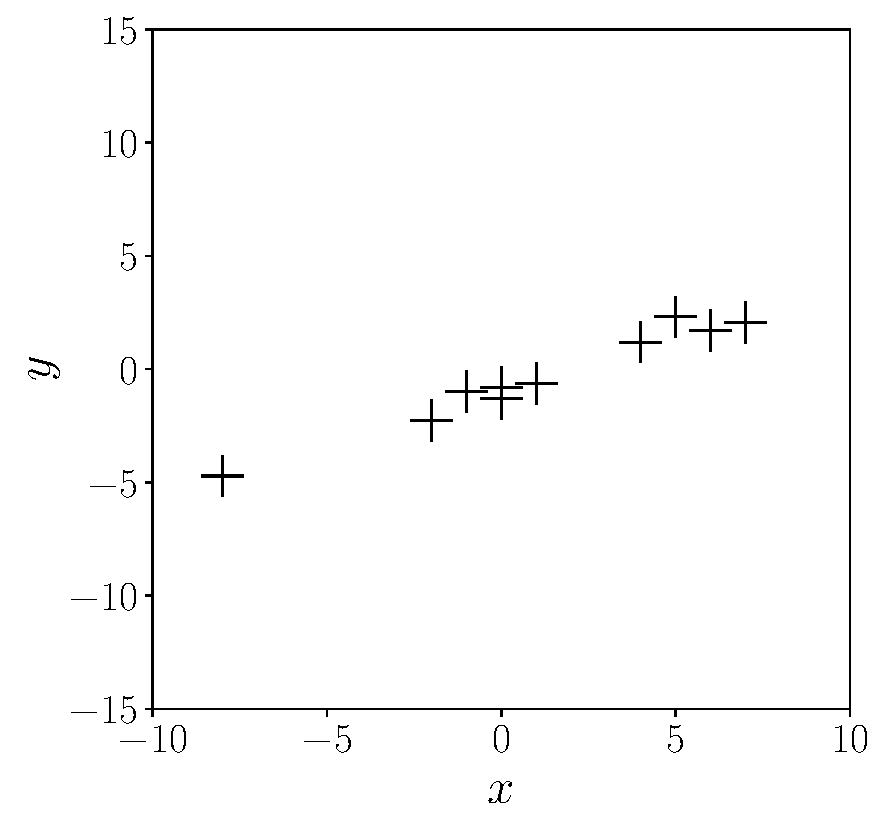
\includegraphics[height = 5cm]{./figures-l11-blr/training_data}
\end{figure}

\end{frame}

\begin{frame}
\frametitle{Sampling from the Posterior  over Functions}
% Good thing: Bayesian linear regression induces a probability
% distribution over functions
Consider a linear regression setting 
\begin{align*}
y &= f(x) + \epsilon =a + bx + \epsilon\,,\quad
  \epsilon\sim\gauss{0}{\sigma_n^2}\\
  p(a,b)& = \gauss{\vec 0}{\mat I}\\
  p(a,b|\mat X, \vec y) & =\gauss{\vec m_N}{\mat S_N} \qquad{\text{Posterior}}
\end{align*}
\end{frame}

\begin{frame}
\frametitle{Sampling from the Posterior  over Functions}
% Good thing: Bayesian linear regression induces a probability
% distribution over functions
Consider a linear regression setting 
\begin{align*}
y &= f(x) + \epsilon =a + bx + \epsilon\,,\quad
    \epsilon\sim\gauss{0}{\sigma_n^2}\\
   [a_i, b_i] &\sim p(a,b|\mat X, \vec y)\\
  f_i &= a_i + b_i x 
\end{align*}
\onslide*<1>{\begin{figure}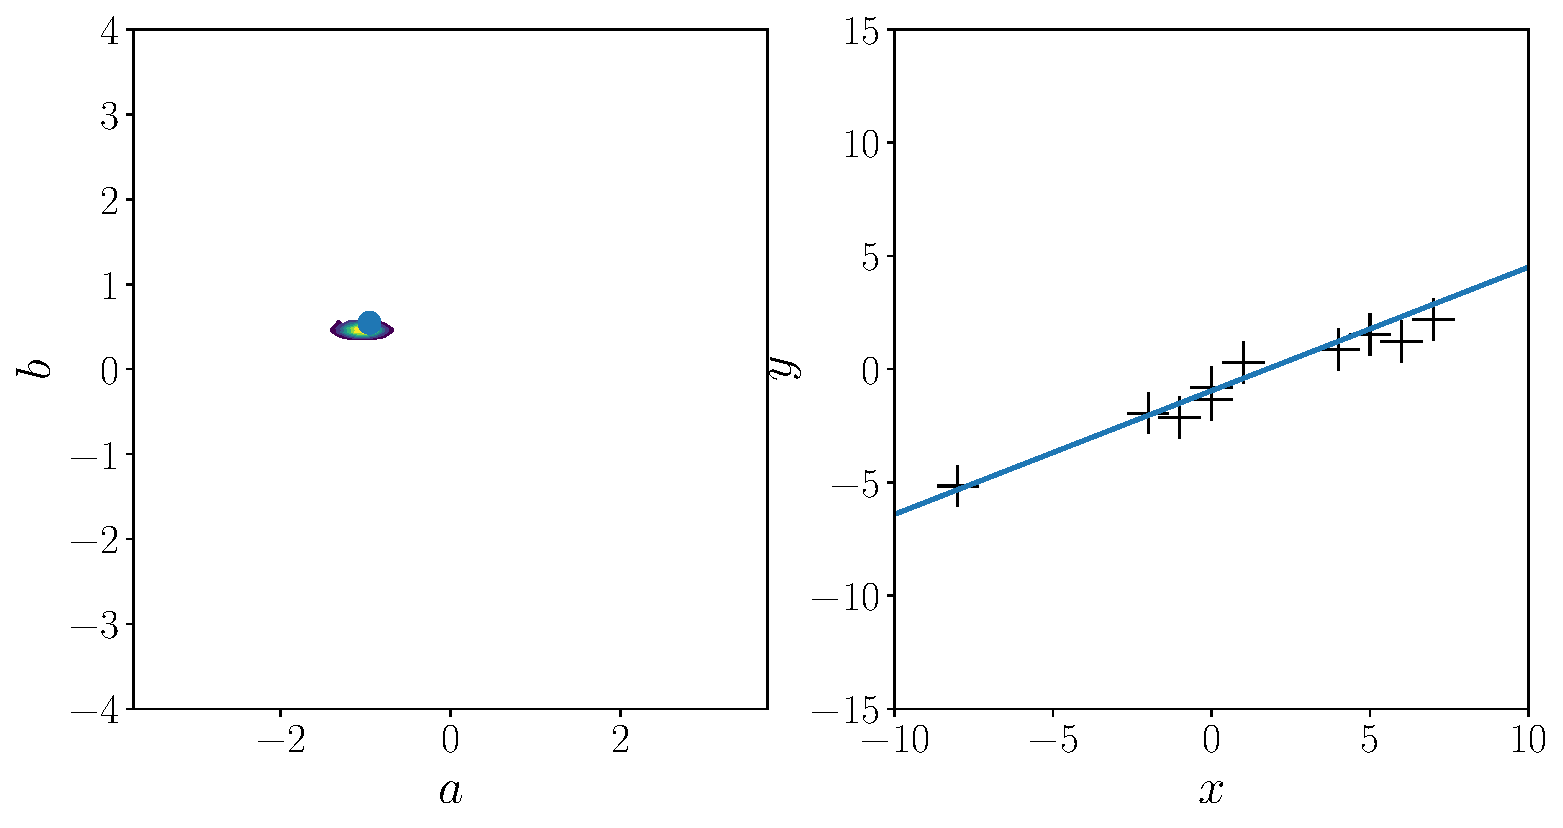
\includegraphics[height = 5cm]{./figures-l11-blr/animation-param-func-dual/posterior_samples_fct_distr_0}\end{figure}}
\onslide*<2>{\begin{figure}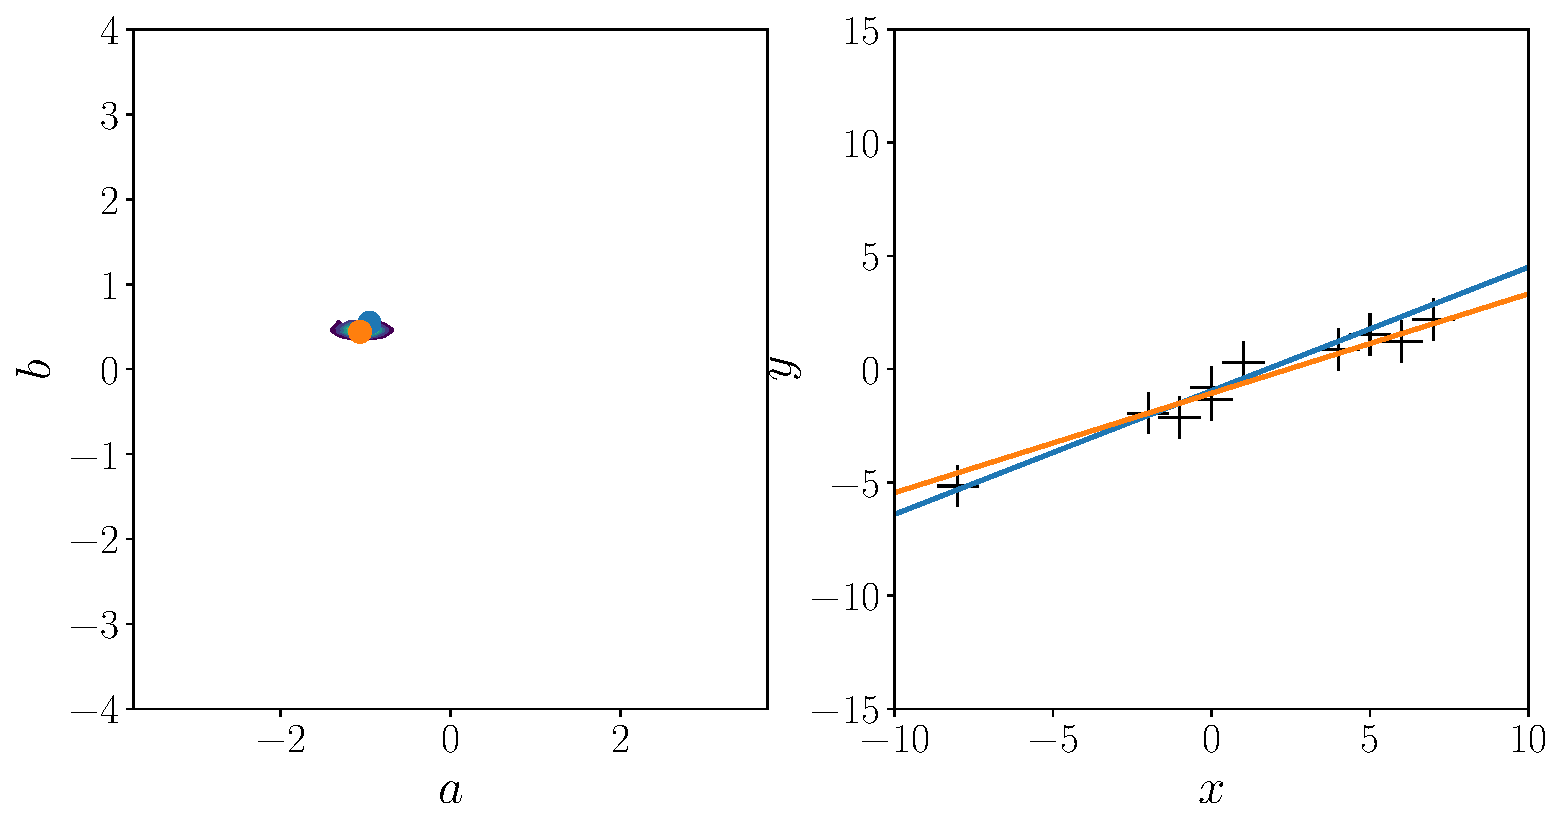
\includegraphics[height = 5cm]{./figures-l11-blr/animation-param-func-dual/posterior_samples_fct_distr_1}\end{figure}}
\onslide*<3>{\begin{figure}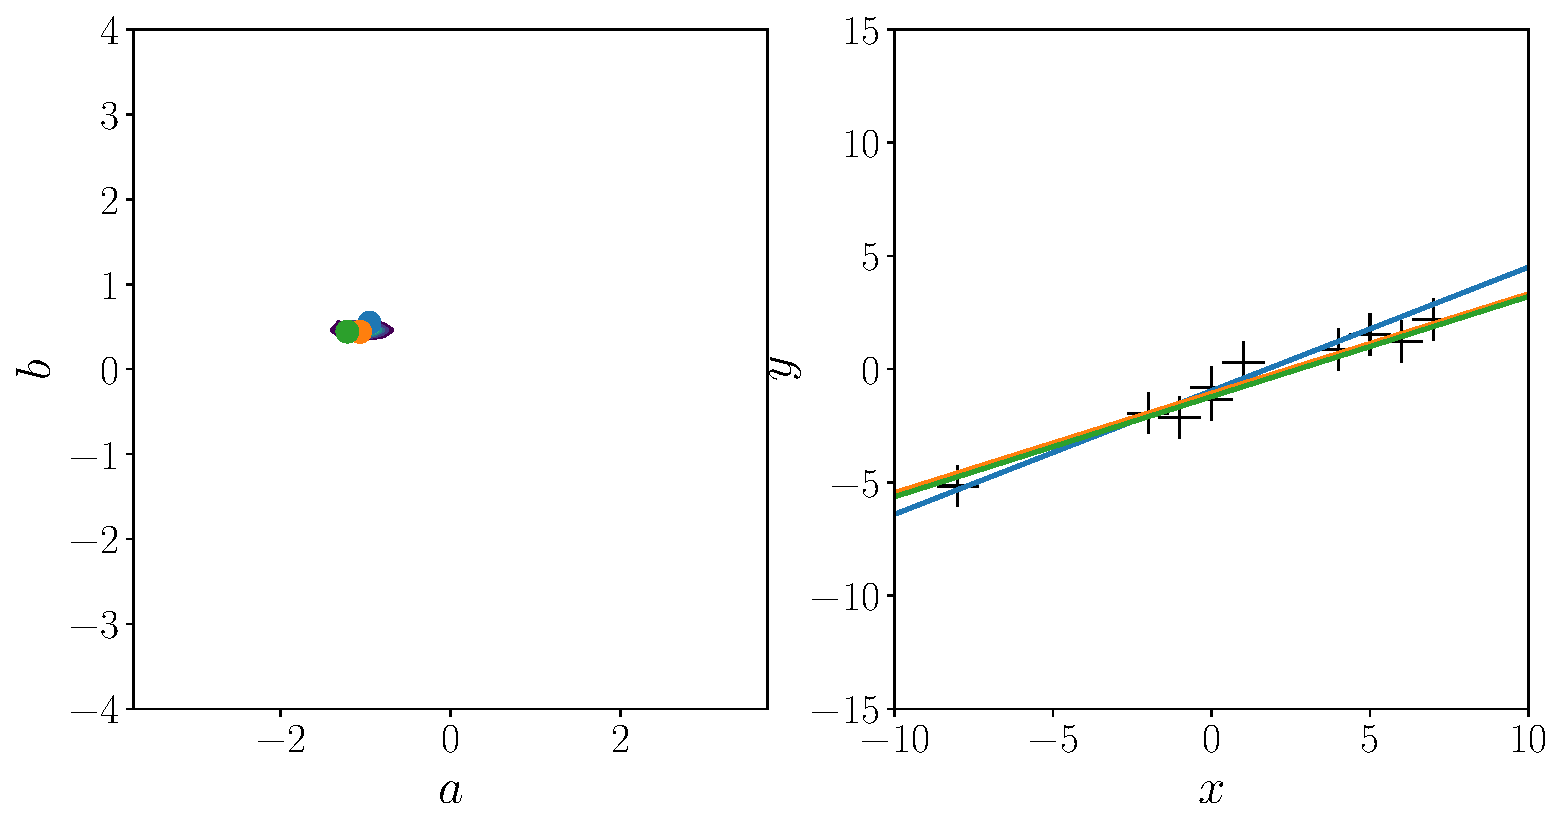
\includegraphics[height = 5cm]{./figures-l11-blr/animation-param-func-dual/posterior_samples_fct_distr_2}\end{figure}}
\onslide*<4>{\begin{figure}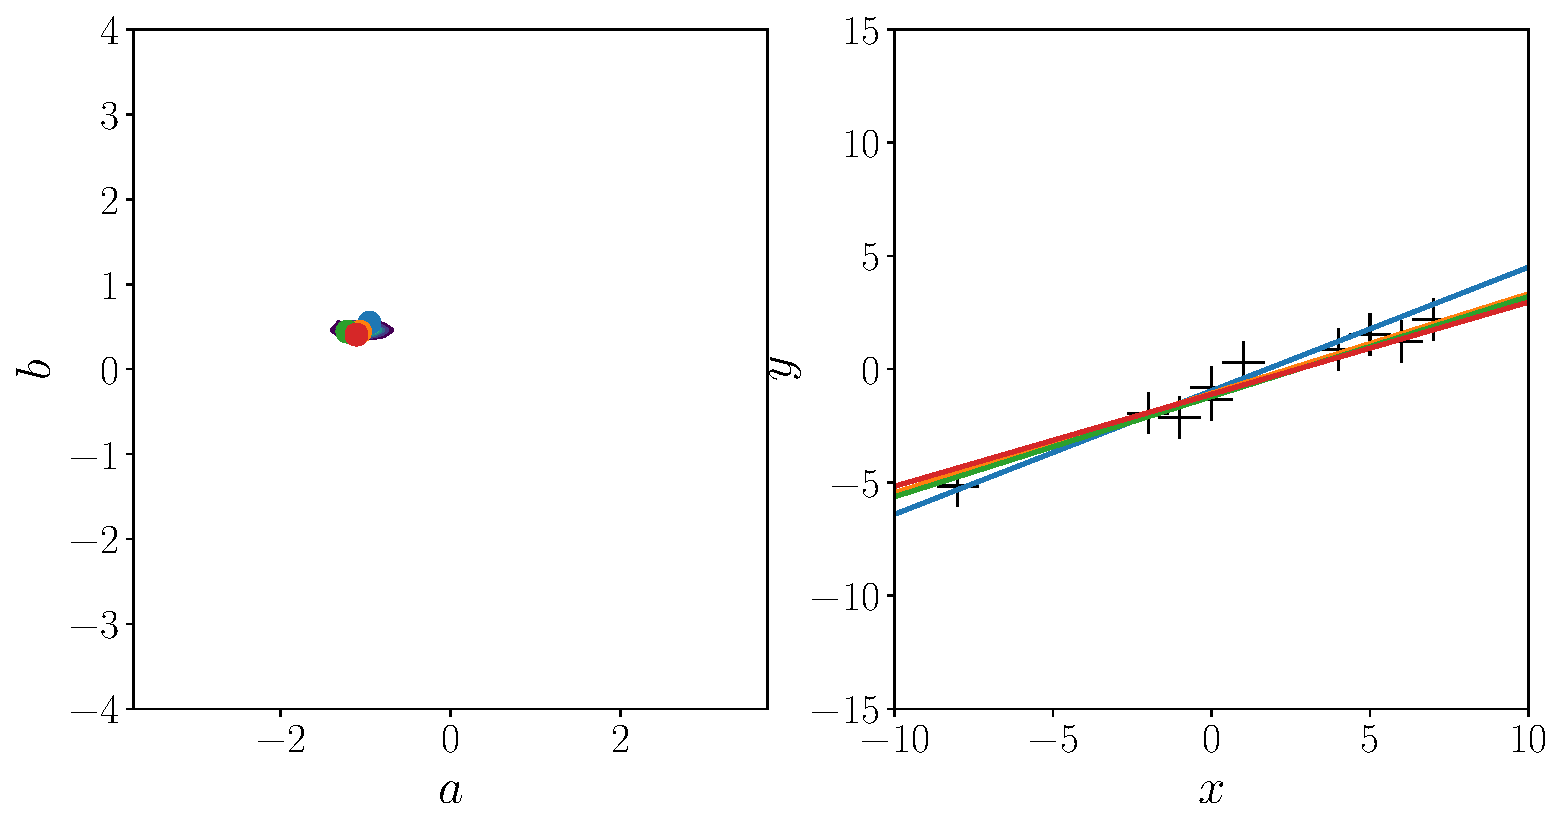
\includegraphics[height = 5cm]{./figures-l11-blr/animation-param-func-dual/posterior_samples_fct_distr_3}\end{figure}}
\onslide*<5>{\begin{figure}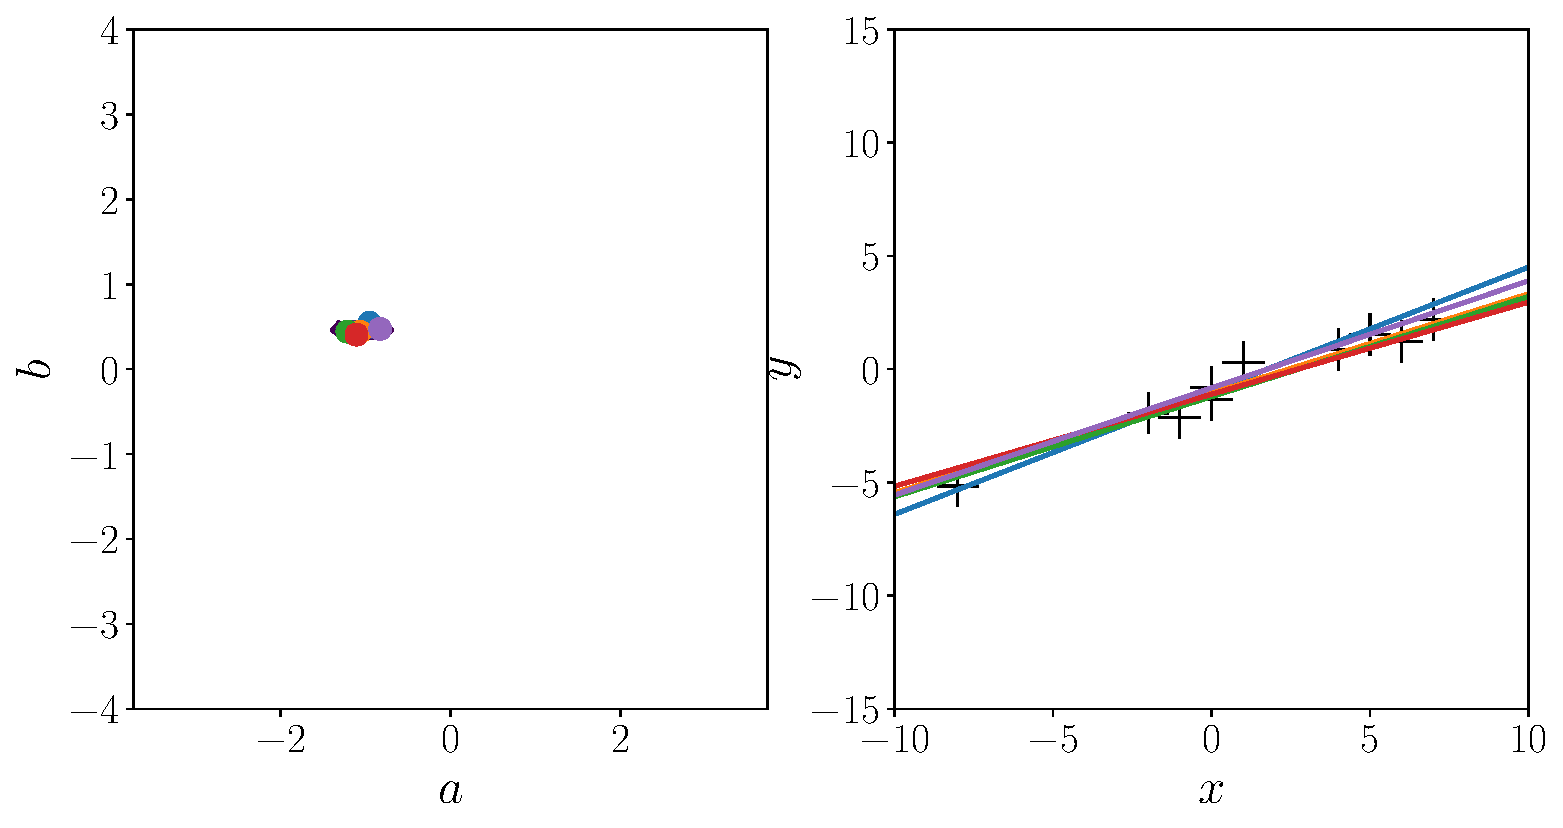
\includegraphics[height = 5cm]{./figures-l11-blr/animation-param-func-dual/posterior_samples_fct_distr_4}\end{figure}}
\onslide*<6>{\begin{figure}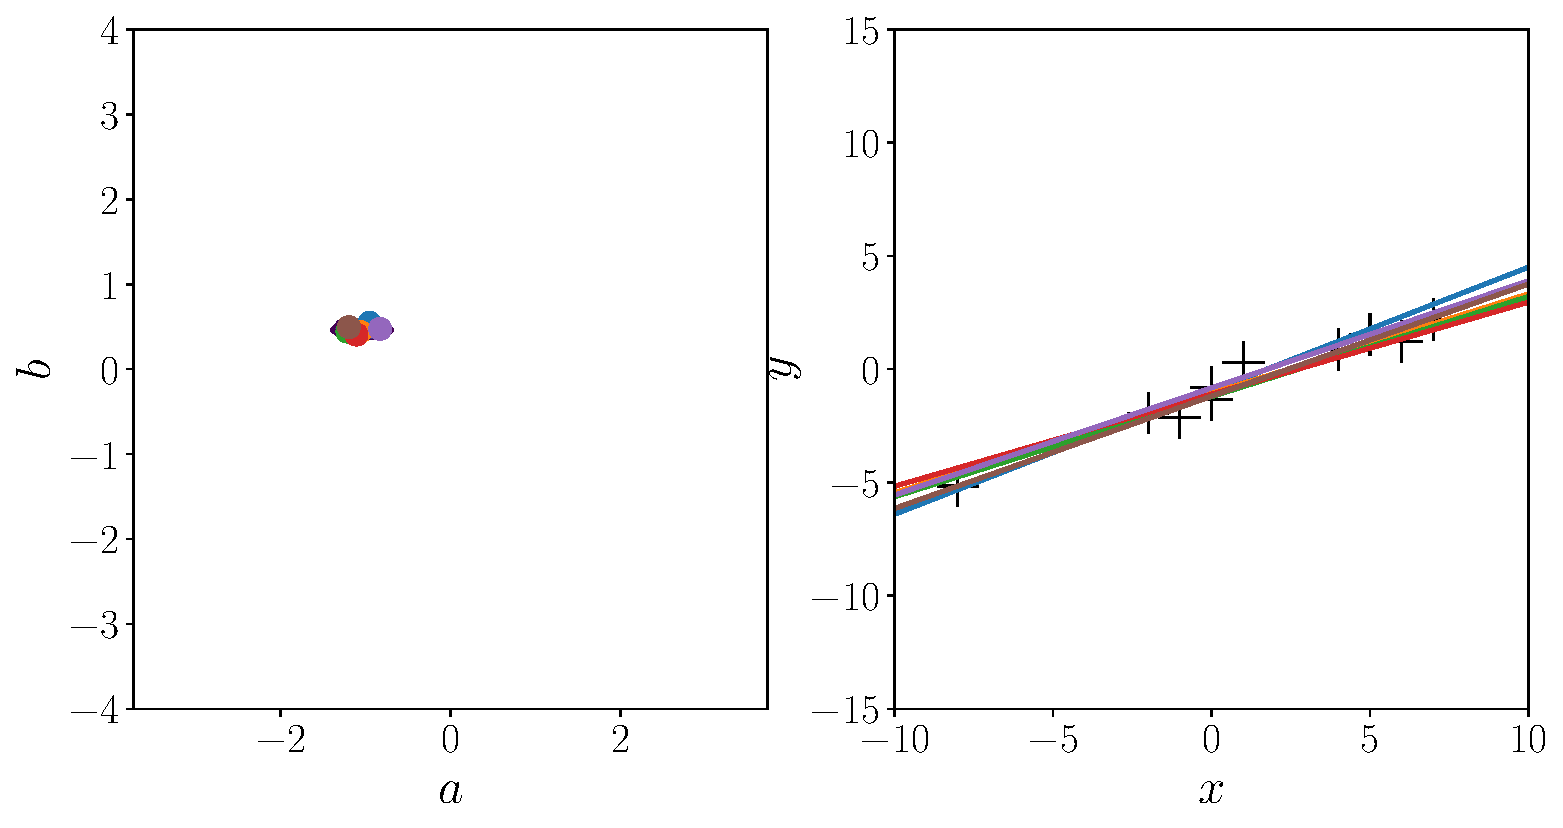
\includegraphics[height = 5cm]{./figures-l11-blr/animation-param-func-dual/posterior_samples_fct_distr_5}\end{figure}}
\onslide*<7>{\begin{figure}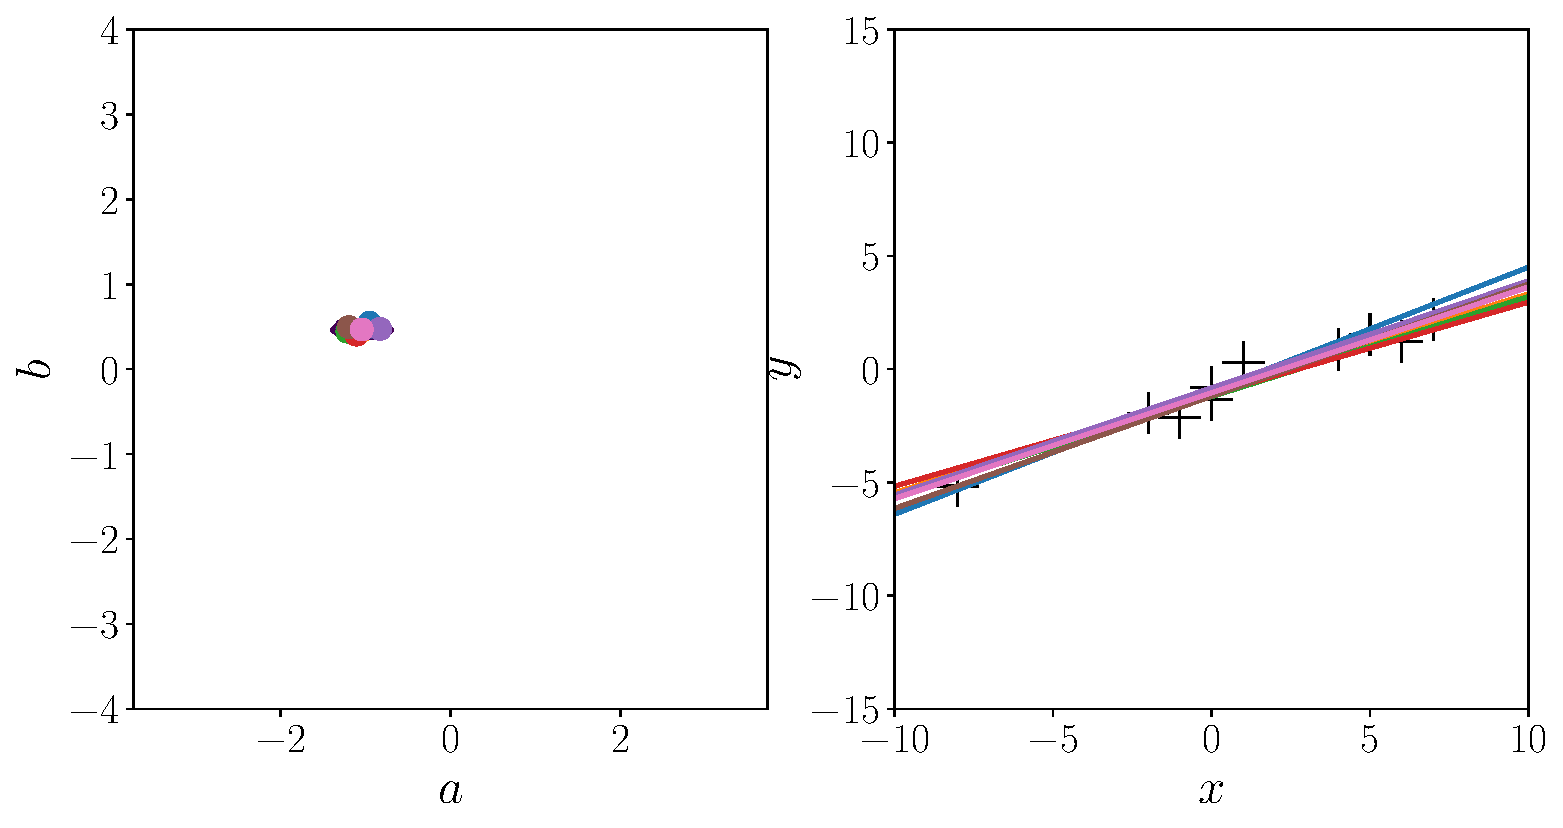
\includegraphics[height = 5cm]{./figures-l11-blr/animation-param-func-dual/posterior_samples_fct_distr_6}\end{figure}}
\onslide*<8>{\begin{figure}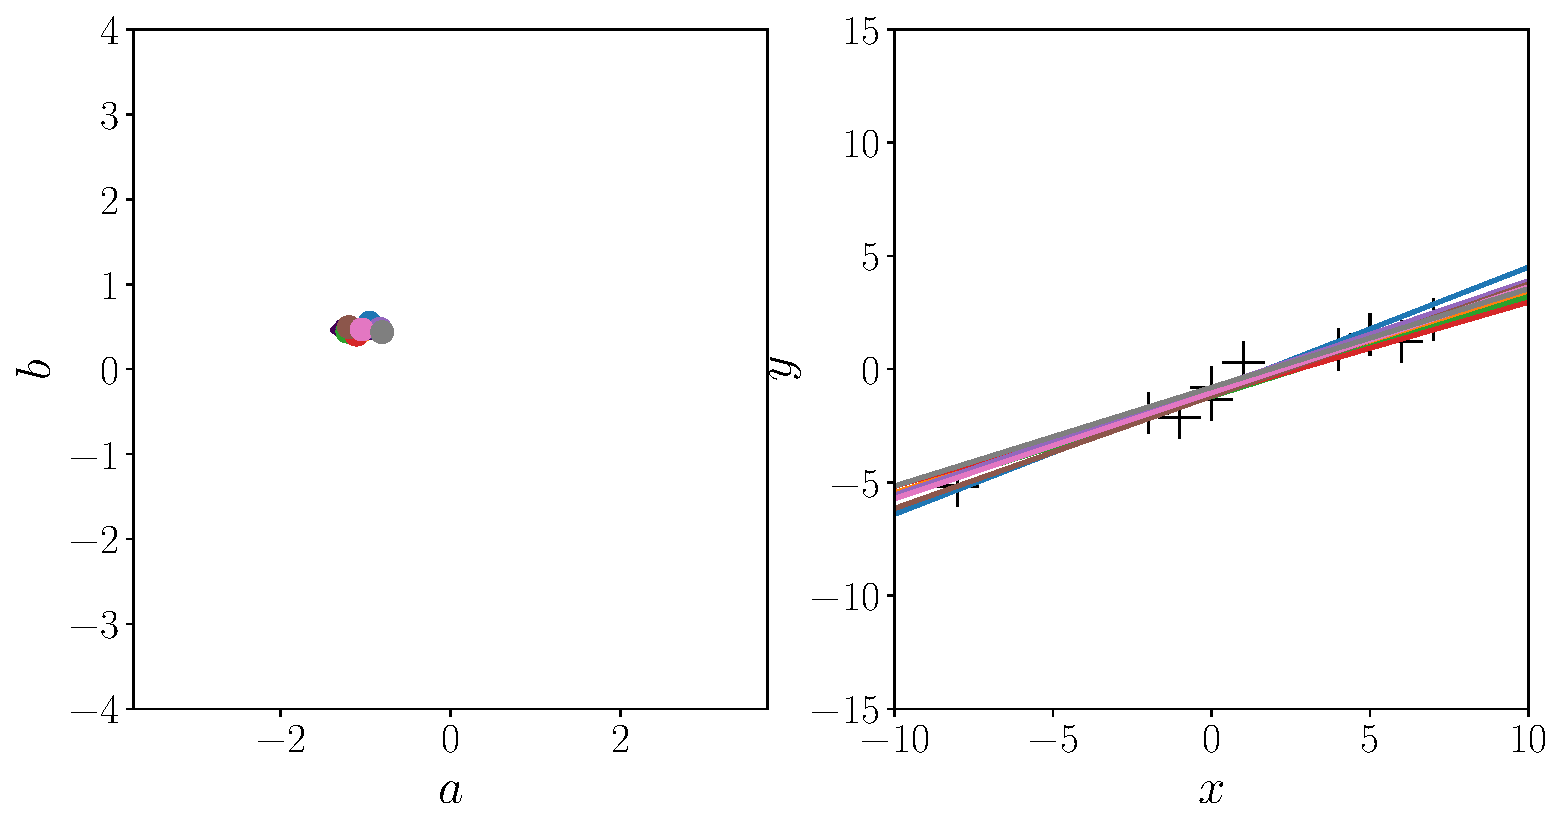
\includegraphics[height = 5cm]{./figures-l11-blr/animation-param-func-dual/posterior_samples_fct_distr_7}\end{figure}}
\onslide*<9>{\begin{figure}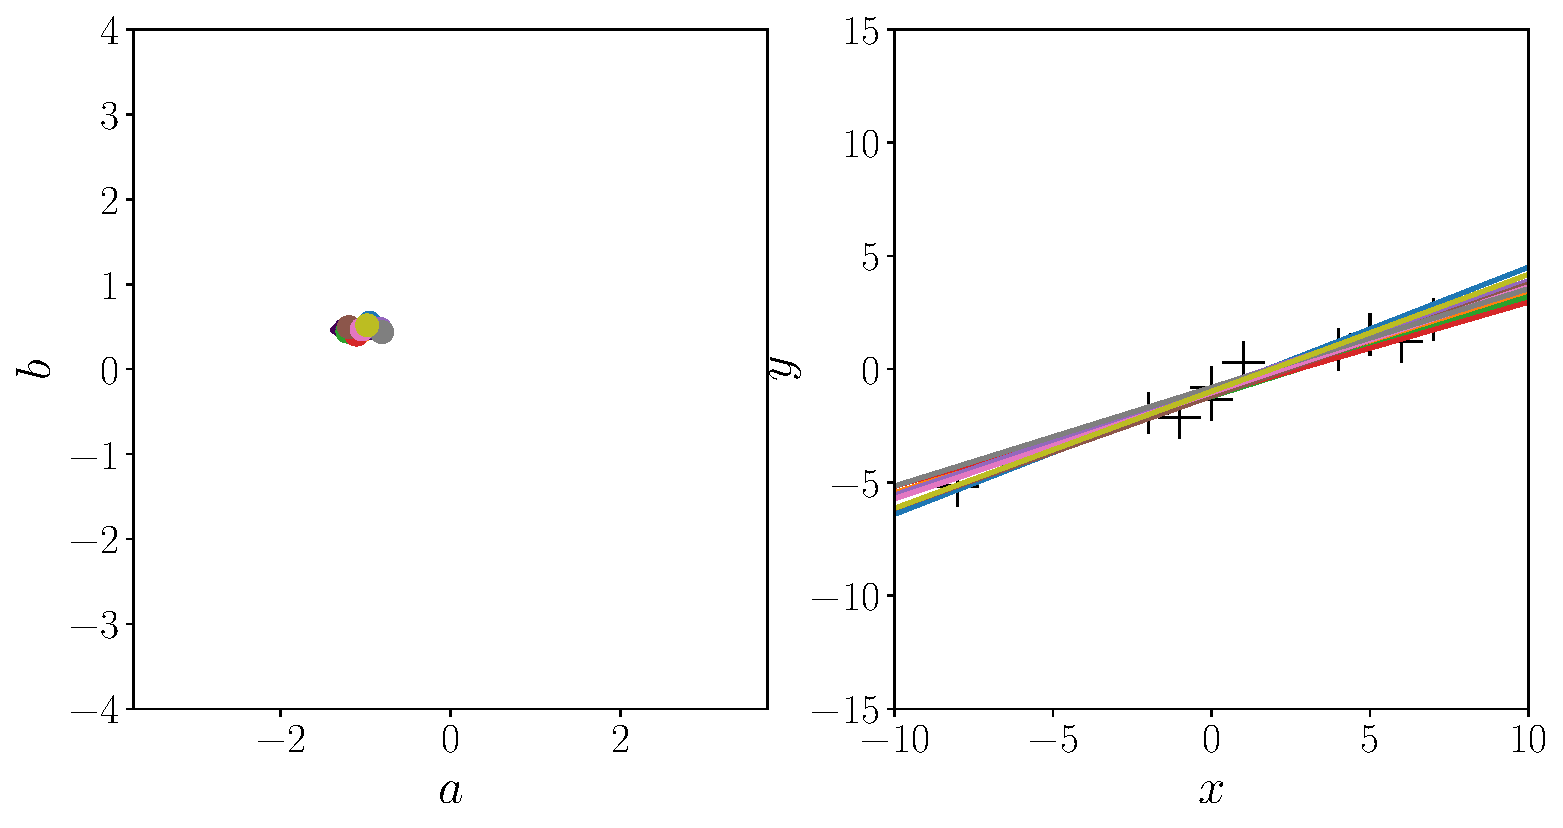
\includegraphics[height = 5cm]{./figures-l11-blr/animation-param-func-dual/posterior_samples_fct_distr_8}\end{figure}}
\onslide*<10>{\begin{figure}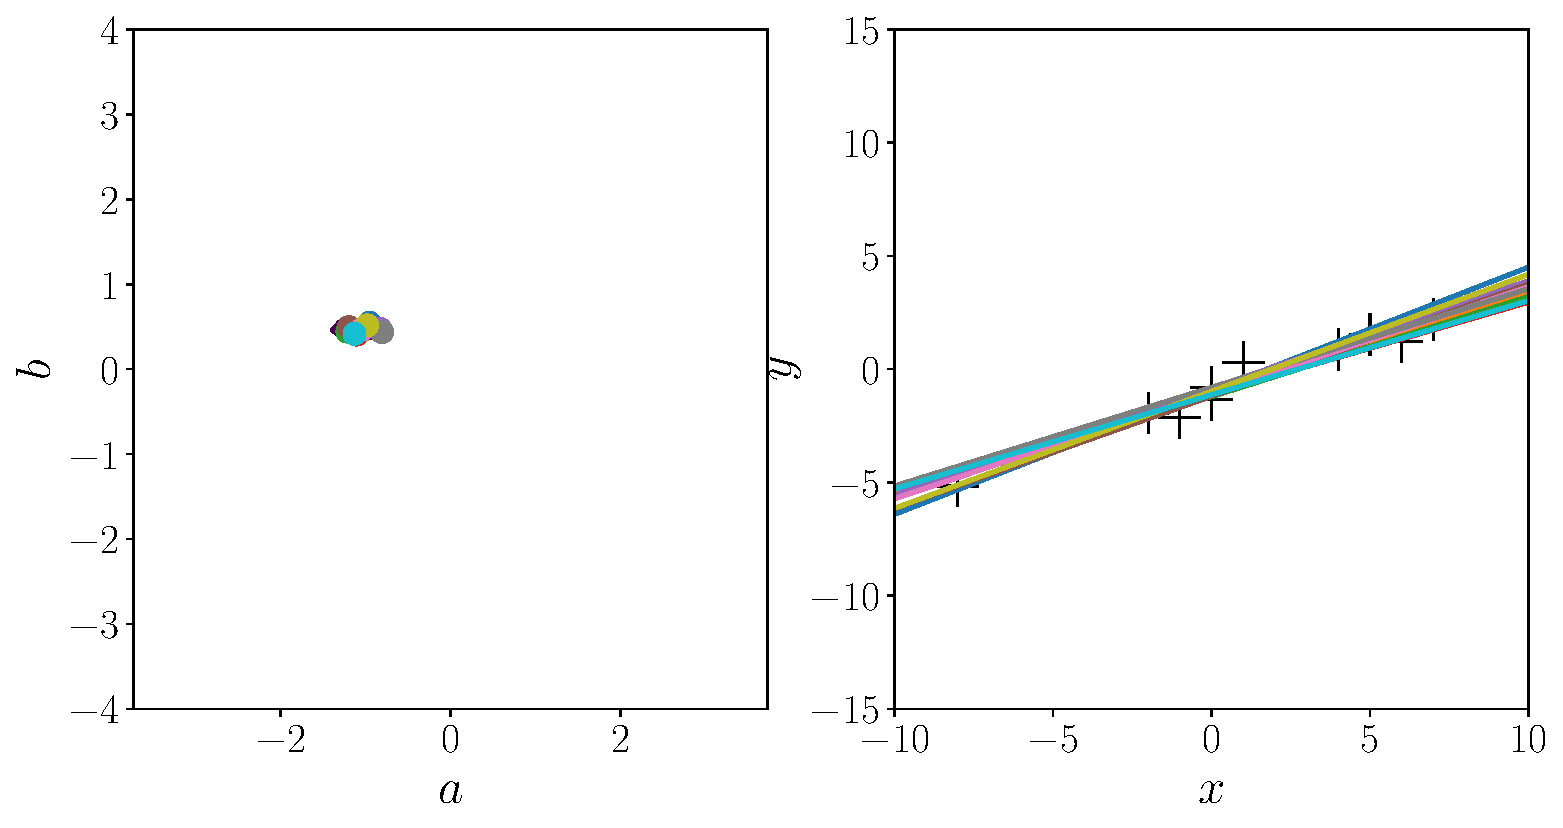
\includegraphics[height = 5cm]{./figures-l11-blr/animation-param-func-dual/posterior_samples_fct_distr_9}\end{figure}}
\end{frame}



\begin{frame}{Model: Bayesian Linear Regression}
We never put a distribution on any $\vx_n$, so we drop from conditioning.
\begin{align}
p(\vtheta)  &= \NormDist{\vtheta; 0, \mathrm I_M} \\
p(y_n|\vtheta) &= \NormDist{y_n; \vphi(\vx_n)\transpose\vtheta, \sigma^2}
\end{align} \pause
\vspace{-0.4cm}
\begin{align}
p(\vy|\vtheta) = \NormDist{\vy; \Phi(\mat X)\vtheta, \sigma^2\mat I_N}
\end{align} \pause

Two goals:
\begin{itemize}
\item Find posterior over parameters $p(\vtheta|\vy)$
\item Find predictive posterior $p(\vy^*|\vy)$
\end{itemize}
\end{frame}

\begin{frame}{Posterior over Parameters}
Board:
\begin{itemize}
\item Equating coefficients (tests your matrix algebra skills!)
\item Joint Gaussian
\item Woodbury identity
\end{itemize}
\end{frame}

\begin{frame}{Method 1: Crunching densities}
\begin{align}
\log p(\vy|\vtheta) &= \log p(\vy|\vtheta) + \log p(\vtheta) \\
&= c - \frac{1}{2\sigma^2}(\vy - \Phi(\mat X)\vtheta)\transpose(\vy - \Phi(\mat X)\vtheta) - \frac{1}{2}\vtheta\transpose\vtheta
\end{align} \pause
This is a vector quadratic in $\vtheta$! {\tiny board} \pause $\implies$ Gaussian. \pause
\begin{itemize}
\item Equate coefficients. Can rearrange... \pause or find $\mathbb E$+$\mathbb V$ by other means \pause
\item Find maximum to find mean {\tiny board} \pause
\item Find Hessian to find covariance {\tiny board} \pause
\end{itemize}
\begin{align}
p(\vtheta|\vy) &= \mathcal{N} \Big(\vtheta; \left[\frac{1}{\sigma^2}\Phi(X)\transpose\Phi(X) + \mat I_M\right]\inv \frac{1}{\sigma^2}\Phi(X)\transpose\vy \\
&\qquad\qquad \left[\frac{1}{\sigma^2}\Phi(X)\transpose\Phi(X) + \mat I_M\right]\inv \Big)
\end{align}
\end{frame}

\begin{frame}{Method 2: Joint Gaussian}
Find
\begin{align}
p(\vtheta,\vy) = \NormDist{\begin{bmatrix}\vtheta \\ \vy\end{bmatrix}; \begin{bmatrix}\Exp{\vtheta}{\vtheta} \\ \Exp{\vy}{\vy}\end{bmatrix}, \begin{bmatrix}\Var{}{\vtheta} & \Cov{}{\theta,\vy} \\ \Cov{}{\vy,\vtheta} & \Var{}{\vy} \end{bmatrix}}
\end{align}

{\tiny board}

\begin{align}
p(\vtheta|\vy) = \mathcal{N}\Big(\vtheta; \Phi(X)\transpose\left[\Phi(X)\Phi(X)\transpose + \sigma^2 \mat I_N\right]\inv\vy, \nonumber \\
 \mat I_M - \Phi(X)\transpose\left[\Phi(X)\Phi(X)\transpose + \sigma^2 \mat I_N\right]\inv\Phi(X)\Big)
\end{align}
\end{frame}

\begin{frame}{Computational Considerations}
Typical algorithms (i.e.~not optimal ones) take:
\begin{itemize}
\item $O(NM^2)$ to multiply matrices of shape $M\times N$ with $N \times M$ \\{\tiny (you must be able to derive this)}
\item $O(N^3)$ to find a matrix inverse
\end{itemize}

\pause
\vspace{0.4cm}
\begin{itemize}
\item The two results are certainly different in computational complexity!
\item From joint is worse when $N\gg M$
\item Are they different in value?
\end{itemize}
\end{frame}

\begin{frame}{Woodbury identity}
\begin{align}
\left(A + UCV\right)\inv = A\inv - A\inv U\left(C\inv + VA\inv U\right)\inv VA\inv
\end{align}

\begin{itemize}
\item Can go back and forth between the two forms.
\item Allows you to implement the most efficient, based on setting of $M$ and $N$.
\item See exercise to practice.
\end{itemize}
\end{frame}

\begin{frame}{Predictive posterior}
{\tiny Board}
\begin{itemize}
\item Crunching densities (see pdf)
\item Equating coefficients (tests your matrix algebra skills!) (see pdf)
\item Joint Gaussian (see exercise)
\item May also need to apply the Woodbury identity
\end{itemize}
\end{frame}

\begin{frame}{Method 1: Crunching densities}
First, how to express our target in terms of densities we know. \pause
\begin{align}
\onslide<2->{p(\vy^*|\vy) &\overset{\text{AT}}{=} \int \frac{p(\vy^*,\vtheta,\vy)}{p(\vy)} \mathrm d\vtheta} \\
\onslide<3->{&\overset{\text{MA}}{=} \int p(\vy^*|\vtheta)\frac{p(\vy|\vtheta)p(\vtheta)}{p(\vy)} \mathrm d\vtheta}
\end{align} \pause \pause
Next do the integrals / equating coefficients. \pause \\
$\implies$ I recommend other method.
\end{frame}



\begin{frame}{Method 2: Expectation identities}
{\tiny board}
\end{frame}




\begin{frame}{Conclusion}
\begin{itemize}
\item Bayesian Linear Regression quantifies uncertainty due to lack of data (epistemic uncertainty)
\item Gaussians are easy to deal with when conditioning
\end{itemize}
\end{frame}





\end{document}
%%% Local Variables: 
%%% mode: latex
%%% TeX-master: t
%%% End: 
